\documentclass{beamer}
\usetheme{Madrid}
\usecolortheme{beaver}
\usepackage[francais]{babel}
\usepackage[utf8]{inputenc} % Required for including letters with accents
\usepackage[T1]{fontenc} % Use 8-bit encoding that has 256 glyphs
\usepackage{pythontex}
\usepackage{amsthm}
\usepackage{amsmath}
\usepackage{amssymb}
\usepackage{mathrsfs}
\usepackage{graphicx}
\usepackage{geometry}
\usepackage{stmaryrd}
\usepackage{tikz}
\usetikzlibrary{patterns}
%\usetikzlibrary{intersections}

\usepackage{stmaryrd}
%\usepackage{tikz}
%\usetikzlibrary{tikzmark}
\usepackage{empheq}
\usepackage{longtable}
\usepackage{booktabs} 
\usepackage{array}
\usepackage{pstricks}
\usepackage{pst-3dplot}
\usepackage{pst-tree}
\usepackage{pstricks-add}
\usepackage{upgreek}
%\usepackage{epstopdf}
\usepackage{eolgrab}
\usepackage{chngpage}
 \usepackage{calrsfs}
 % Appel du package pythontex 
\usepackage{pythontex}





\usetikzlibrary{decorations.pathmorphing}
\def \de {{\rm d}}
\usepackage{color}
\usepackage{xcolor}
\newcommand{\mybox}[1]{\fbox{$\displaystyle#1$}}
\newcommand{\myredbox}[1]{\fcolorbox{red}{white}{$\displaystyle#1$}}
\newcommand{\mydoublebox}[1]{\fbox{\fbox{$\displaystyle#1$}}}
\newcommand{\myreddoublebox}[1]{\fcolorbox{red}{white}{\fcolorbox{red}{white}{$\displaystyle#1$}}}
%\usetheme[options]{Boadilla}

  \title{Méthode des éléments finis}
  \author{ \textsc{Ibrahim ALAME}}\institute{ESTP}
\date{19/10/2022}
  \begin{document}
 \begin{frame}
  \titlepage
  \end{frame}
  
\begin{frame}
\frametitle{Éléments finis d'Hermite}
$\varphi_i$ des éléments finis de Lagrange est construite pour être continue d'un élément à l'autre, mais pas sa dérivée... 

Un élément fini d'Hermite est un triplet $(K,\Sigma,P)$ tel que :
\begin{itemize}
\item K est un élément géométrique de $\mathbb{R}^n$, compact, connexe, et d'intérieur non vide ;
\item $\Sigma=\{\sigma_1,\cdots,\sigma_N\}$ un ensemble de $N$ formes linéaires sur l'espace des fonctions définies sur $K$, ou sur un sous-espace plus régulier contenant $P$ ;
\item $P$ est un espace vectoriel de dimension finie de fonctions réelles définies sur $K$, et tel que $\Sigma$ soit $P-$unisolvant.
\end{itemize}
\end{frame}
%%%%%%%%%%%%%%%%%%%%%%%%%%%%%%%%%%%%%%%%%%%%%%%%%%%%%%%
\begin{frame}
\frametitle{Opérateur de $P-$interpolation }


\begin{itemize}
\item Un opérateur de $P-$interpolation sur $\Sigma$ est un opérateur $\Pi$ qui à toute fonction $v$ définie sur $K$ associe la fonction $\Pi v$ de P définie par :
\[\Pi v=\sum_{i=1}^N\sigma_i(v)\varphi_i\]
\item $\Pi v$  est l'unique élément de $P$ qui prend les mêmes valeurs que $v$ sur les points de $\Sigma$.
\item
\[\sigma_j(\varphi_i)=\delta_{ij},\quad 1\leq i,j \leq N\]
\item Suivant les éléments utilisés, ces fonctions de base pourront être de classe $C^1$ ou même plus, et il en sera donc de même pour la solution approchée $u_h$.
\end{itemize}

\end{frame}

%%%%%%%%%%%%%%%%%%%%%%%%%%%%%%%%%%%%%%%
\begin{frame}
\frametitle{Éléments unidimensionnels}

\begin{center}
\begin{tikzpicture}[domain=0:5,scale=0.50]
  \draw[-] (0,0) -- (6,0);
  \node [gray] at (0,0) {$\bullet$};
\draw (0,0) circle (0.3);
  \node [gray] at (6,0) {$\bullet$};
\draw (6,0) circle (0.3);

  \draw[-] (8,0) -- ++(6,0);
  \node [gray] at (8,0) {$\bullet$};
\draw (8,0) circle (0.3);
\draw (8,0) circle (0.5);
  \node [gray] at (8+6,0) {$\bullet$};
\draw (8+6,0) circle (0.3);
\draw (8+6,0) circle (0.5);
\end{tikzpicture}

\end{center}

\begin{center}
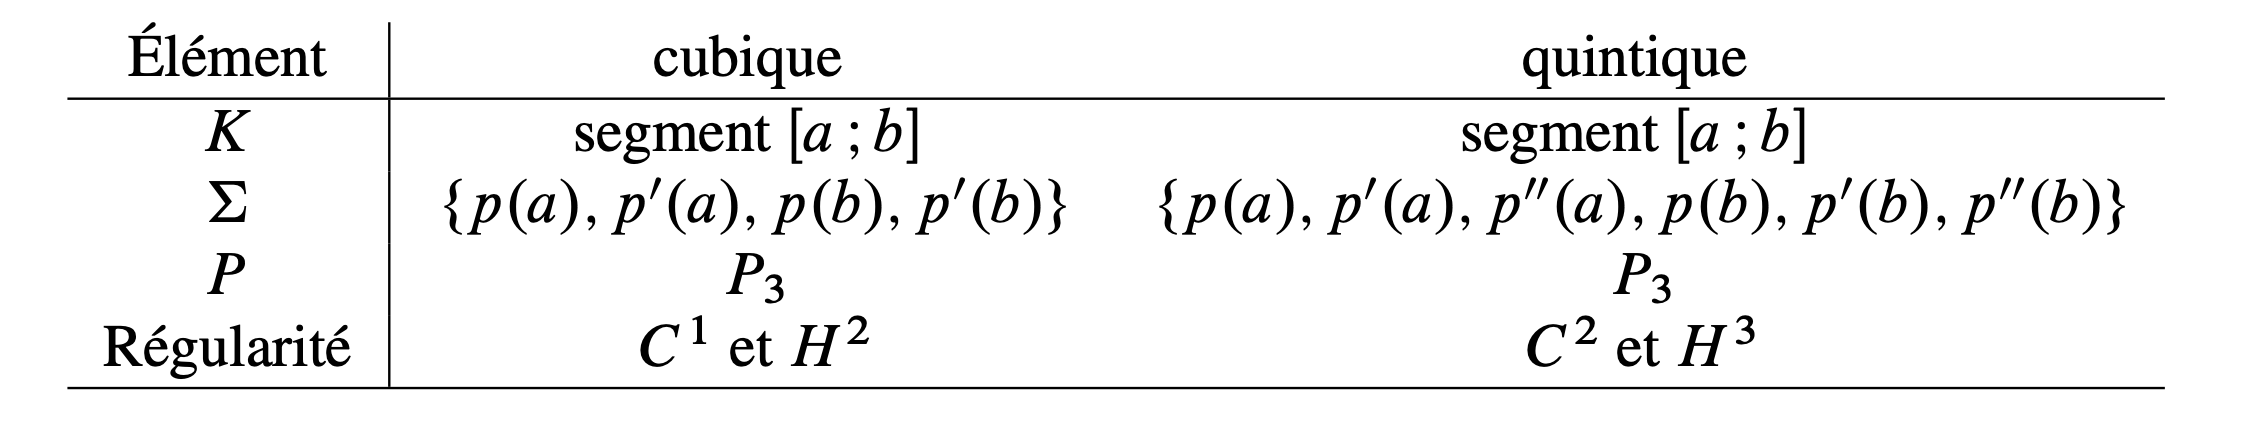
\includegraphics[scale=0.3]{hermite3-5.png} 
\end{center}
\begin{center}
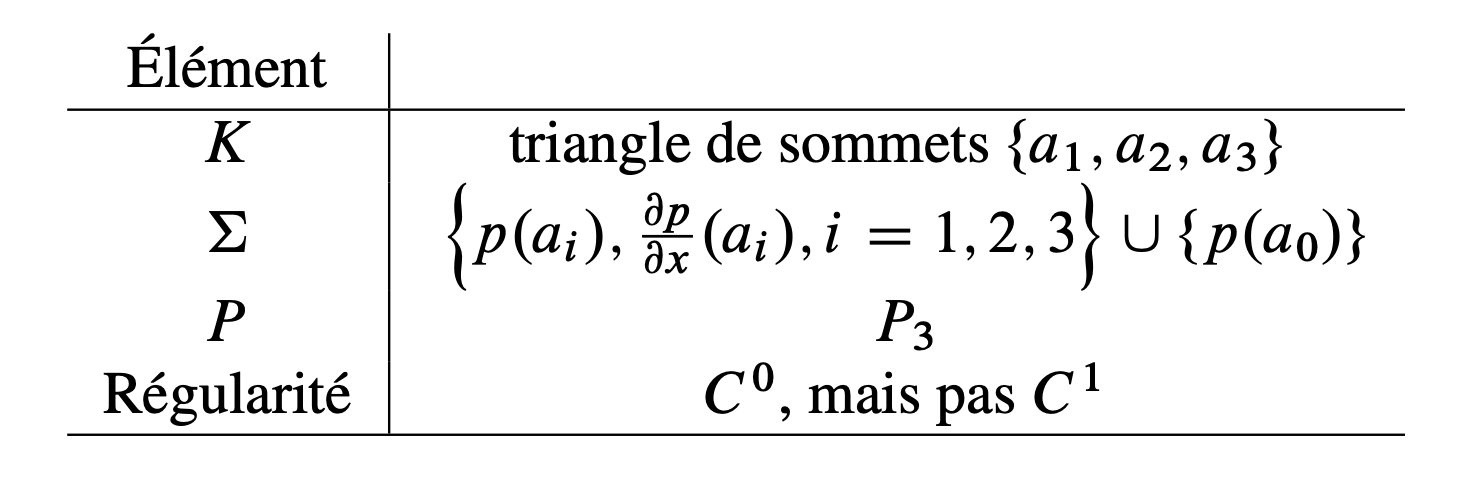
\includegraphics[scale=0.3]{hermiteTriangle1.png} 
\end{center}
\end{frame}
%%%%%%%%%%%%%%%%%%%%%%%%%%%%%%%%%%%%%%%
\begin{frame}
\frametitle{Élément triangle}


\begin{center}
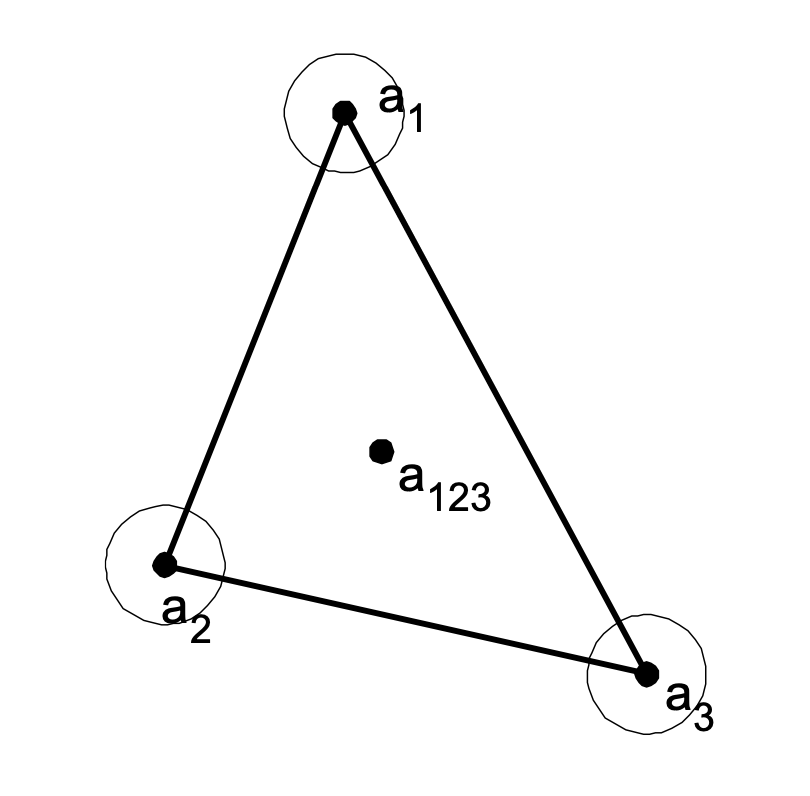
\includegraphics[scale=0.3]{hermiteTriangleUN.png} 
\end{center}
\begin{center}
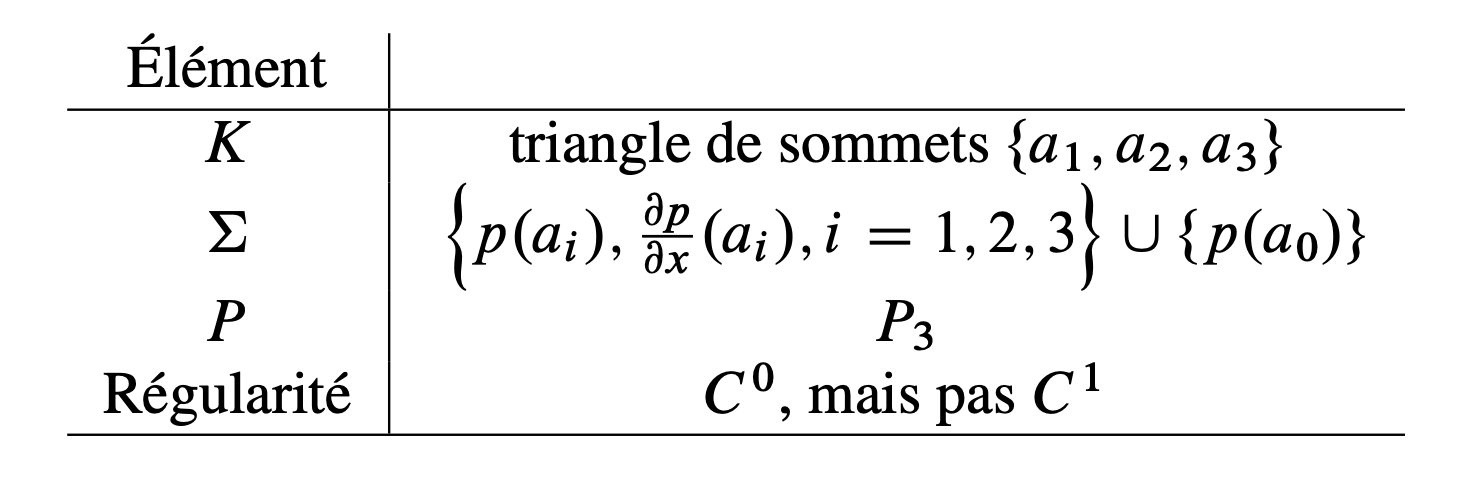
\includegraphics[scale=0.3]{hermiteTriangle1.png} 
\end{center}
\end{frame}
%%%%%%%%%%%%%%%%%%%%%%%%%%%%%%%%%%%%%%%
\begin{frame}
\frametitle{Éléments bidimensionnels}
\begin{center}
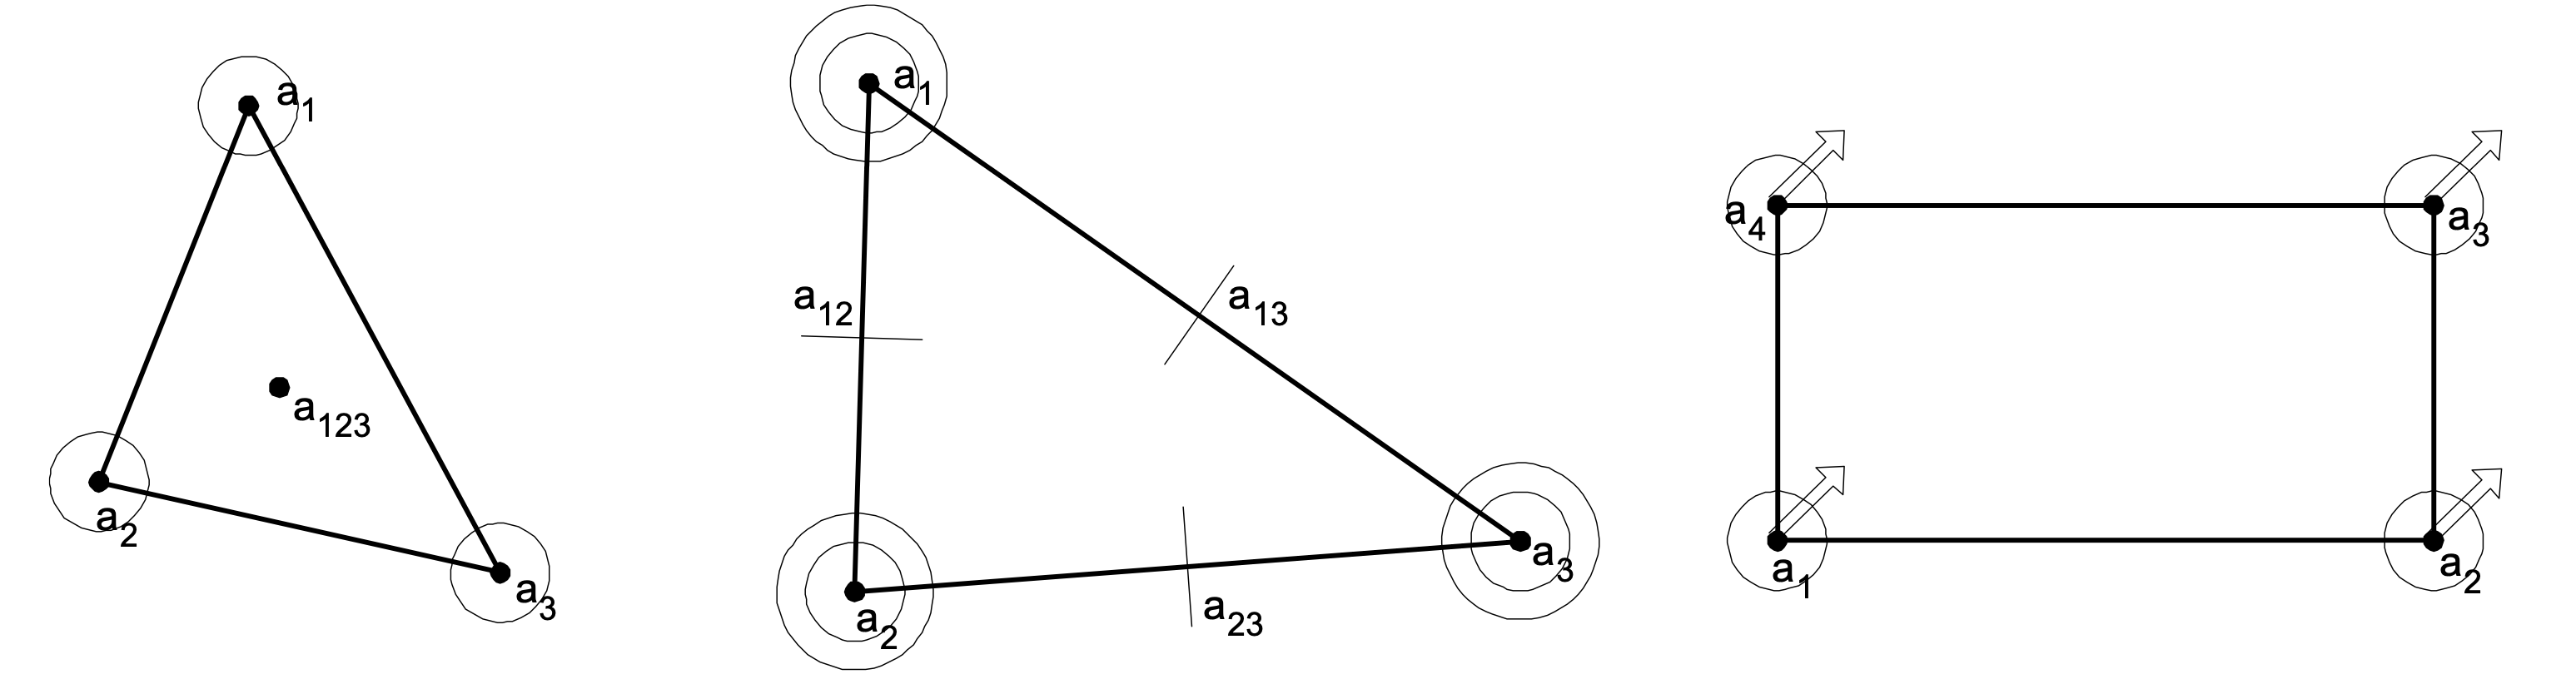
\includegraphics[scale=0.2]{elementsHermite.png} 
\end{center}
\begin{center}
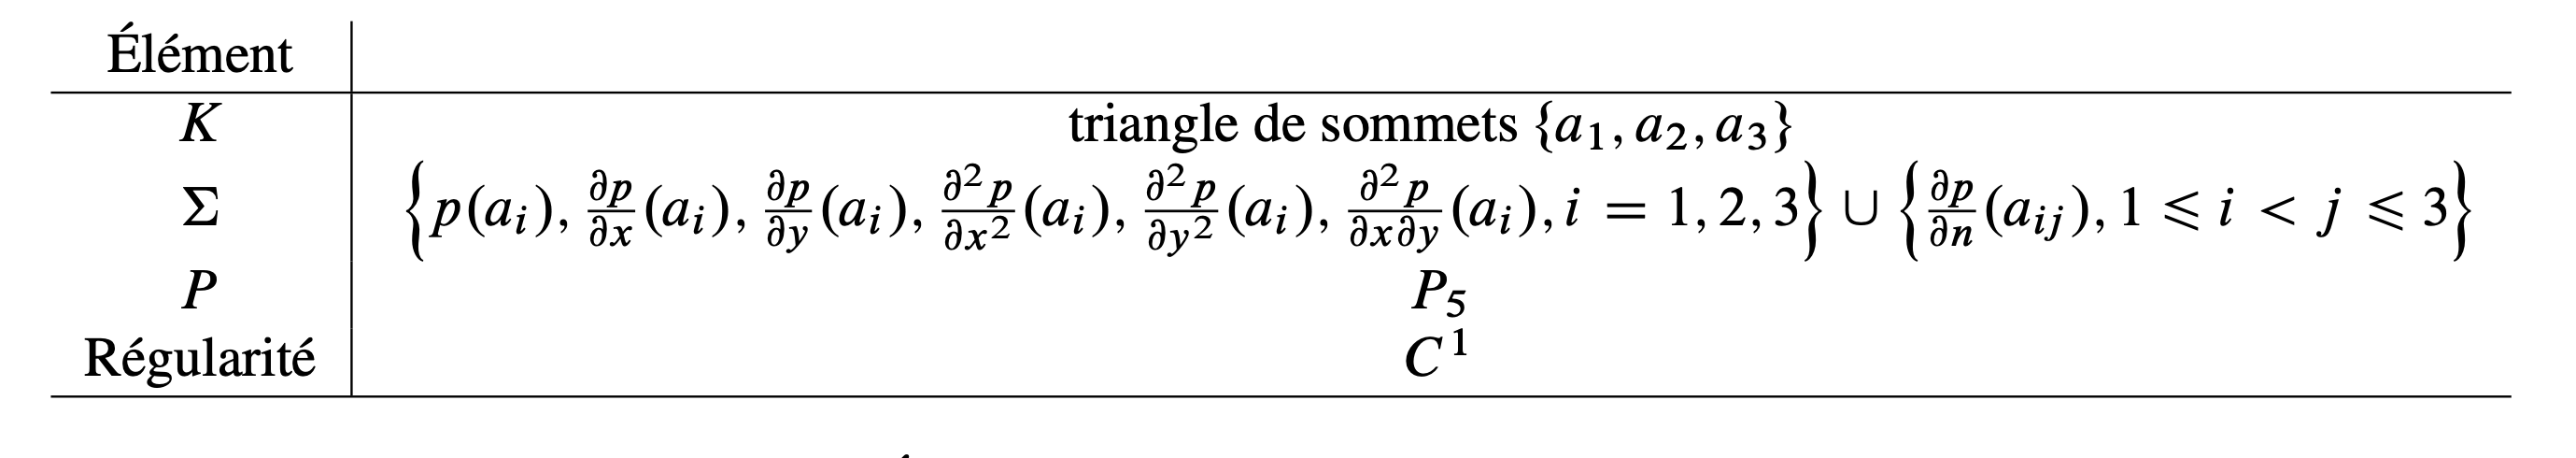
\includegraphics[scale=0.25]{hermiteBidim1.png} 
\end{center}
\begin{center}
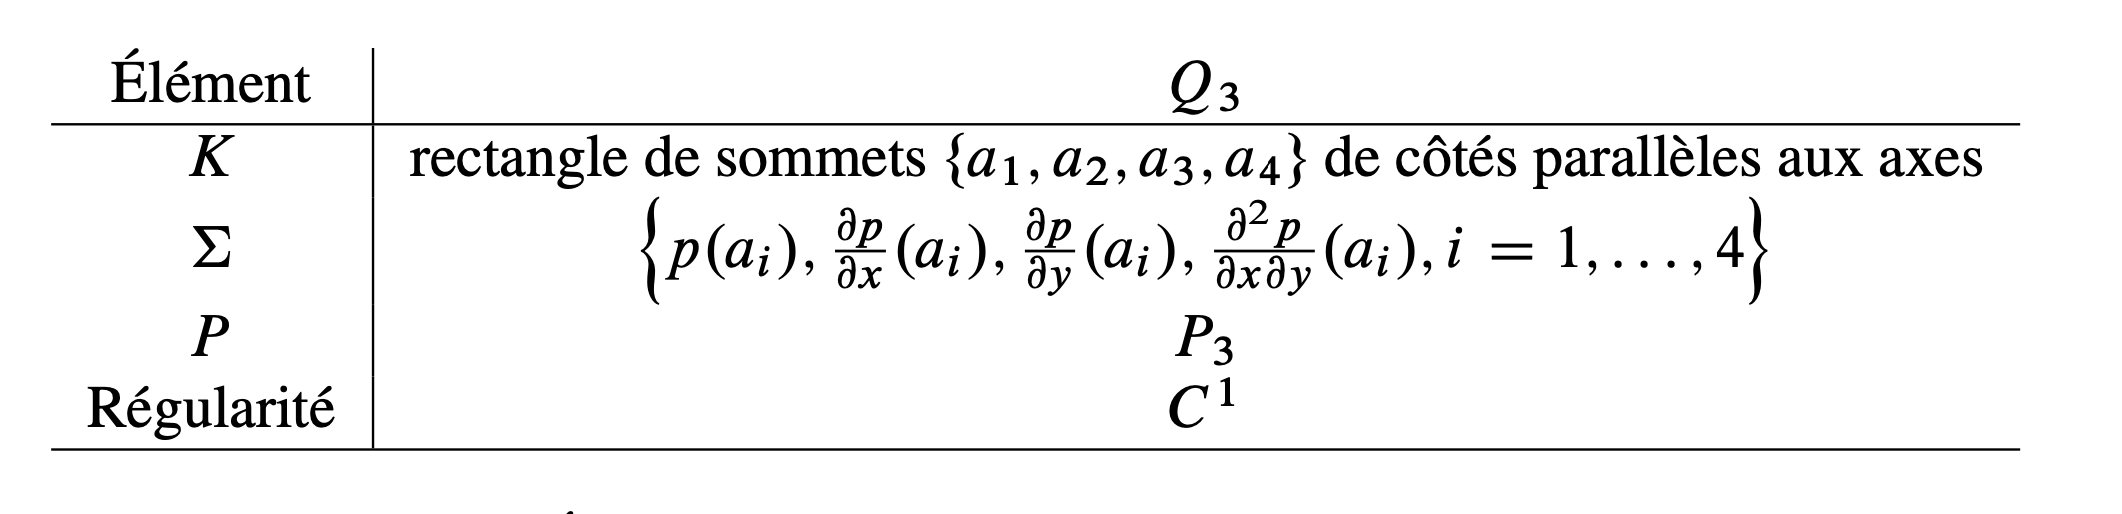
\includegraphics[scale=0.25]{hermiteBidim2.png} 
\end{center}

\end{frame}



\begin{frame}
\frametitle{Les fonctions de base}

\begin{itemize}
\item $\Phi_{i}(x)$ les fonctions de base associées aux valeurs nodales de la fonction $v_{i}$.
\item $\Psi_{i}(x)$ les fonctions de base associées aux valeurs nodales de la dérivée $(\frac{dv}{dx})_{i}$,
\end{itemize}


\begin{displaymath}
\Pi v (x)=\sum_{i=1}^{n}v_{i}\Phi_{i}(x)+\sum_{i=1}^{n}(\frac{dv}{dx})_{i}\Psi_{i}(x)\end{displaymath}

Sur un élément $[x_{1},x_{2}]$, cette approximation s'écrit:

\begin{displaymath}
v^{h}(x)=v_{1}\Phi_{1}(x)+(\frac{dv}{dx})_{1}\Psi_{1}(x)+v_{2}\Phi_{2}(x)+(\frac{dv}{dx})_{2}\Psi_{2}(x)\end{displaymath}

$\Phi_{i}$ et $\Psi_i$ vérifient les conditions:
\[\left\{\begin{array}{l}
\Phi_{i}(x_j)=\delta_{ij}\quad \Phi'_{i}(x_j)=0\\
\Psi_{i}(x_j)=0\quad \Psi'_{i}(x_j)=\delta_{ij}
\end{array} \right. \]
\end{frame}



\begin{frame}
\frametitle{Les fonctions de base}
\[\left\{\begin{array}{l}
\Phi_i(x) = \left[1-2(x-x_i)\lambda'_i(x_i)\right]\lambda^2_i(x) \\
\Psi_i(x) = (x-x_i)\lambda^2_i(x) 
\end{array}\right.
 \]
 \begin{itemize}
 \item élément de référence de longueur $h$:  $x_1=0$ et $x_2=h$, 
 \item $\lambda_1(x)=1-\frac{x}{h}$ et $\lambda_2(x)=\frac{x}{h}$. On pose $\xi= \frac{x}{h}$:
 \[\left\{\begin{array}{l}
\Phi_1(x) = (1+2\xi)(1-\xi)^2 \\
\Phi_2(x) = (3-2\xi)\xi^2 \\
\Psi_1(x) = h \xi(1-\xi)^2\\
\Psi_2(x) = h (\xi-1)\xi^2
\end{array}\right.
 \]
 \begin{center}
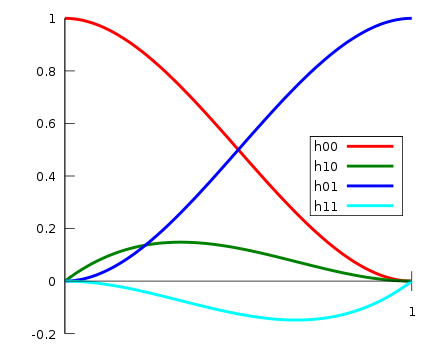
\includegraphics[scale=0.25]{HermiteBasis.png} 
\end{center}
 \end{itemize}

\end{frame}





%%%%%%%%%%%%%%%%%%%%%%%%%%%%%%%%%%%%%%%%%%
\begin{frame}
\frametitle{Structure de données d'un maillage}
{\huge Liste des sommets}
\begin{itemize}
\item  $N_s$ nombre des sommets,
\item  Pour chaque sommet $i=1,\cdots, N_s$,
    \begin{itemize}
        \item les coordonnées du sommet $i$.
     \end{itemize}
\item Exemples en dimension 1: $a=x_0<x_1<x_2<\cdots<x_n=b$
\begin{itemize}
\item $N_s=n+1$
\item Tableau à une entrée de longueur $N_s$
\begin{center}
\begin{tabular}{|c|c|c|c|c|}\hline 
{\bf i} & 1 & 2 & ... & $N_s$ \\ \hline 
{\bf x} & $x_0$ & $x_1$ & ... & $x_n$ \\ \hline 
\end{tabular}
\end{center}
Il ne faut pas toujours stocker cette structure de données. Si la grille est uniforme, elle est donnée de façon implicite par
\[N_s=n+1;\; h=\frac{1}{n}\quad x_0=a;\; x_i=a+x_0+ih,\; i=1,\cdots,(N_s-1).\]
\end{itemize}
\end{itemize}
\end{frame}
%%%%%%%%%%%%%%%%%%%%%%%%%%%%%%%%%%%%%%%%%%%%%
\begin{frame}
\frametitle{Liste des sommets en dimension 2}
 Tableau des coordonnées $\{(x_{1i},x_{2i})\}_{i=1}^{N_s}$.
 \begin{itemize}
 \item Nombre de sommets : $N_s$
 \item Tableau à deux lignes et $N_s$ colonnes
 \begin{center}
\begin{tabular}{|c|c|c|c|c|}\hline 
{\bf i} & 1 & 2 & ... & $N_s$ \\ \hline 
$\mbox{\bf x}_{1i} $& $x_{11}$ & $x_{12}$ & ... & $x_{1n}$ \\ \hline 
$\mbox{\bf x}_{2i} $& $x_{21}$ & $x_{22}$ & ... & $x_{2n}$ \\ \hline 
\end{tabular}
\end{center}
\begin{tabular}{cc}
\begin{tikzpicture}[domain=0:5,scale=0.50]
  \draw[->] (-1,0) -- (6,0)node[right]{$x$};
  \draw[->] (0,-1) -- (0,6)node[left]{$y$};
  \draw[->] (0,0) -- ++(5,0) -- ++(0,5) -- ++(-5,0) --cycle ;
  \node [gray] at (0,0) {$\bullet$};
  \node [gray] at (5,0) {$\bullet$};
  \node [gray] at (0,5) {$\bullet$};
  \node [gray] at (5,5) {$\bullet$};
  \draw [red] (0,0) node[below right]{1};
  \draw [red](5,0) node[below]{2};
  \draw [red] (5,5) node[right]{3};
  \draw [red]  (0,5) node[above right]{4};
  \draw[->] (0,0) -- ++(5,5) ;
   \draw[->] (0,5) -- ++(5,-5) ;
   \node [gray] at (2.5,2.5) {$\bullet$};
   \draw [red] (2.5,2.5)node[above] {5};
\end{tikzpicture}
&
\begin{tabular}{|c|c|c|c|c|c|}\hline 
{\bf i} & 1 & 2 & 3& 4&5 \\ \hline 
$\mbox{\bf x}_{1i} $& 0 & $L$ & $L$ & 0 &$L/2$\\ \hline 
$\mbox{\bf x}_{2i} $& 0 & 0     & $H$ & $H$ &$H/2$\\ \hline 
$\Gamma$& 1 & 1 & 1 & 1&0 \\ \hline 
\end{tabular}
\end{tabular}
 \end{itemize}



\end{frame}

\begin{frame}
\frametitle{Table de connectivité}
\begin{itemize}
\item  $N_e$ nombre d'éléments,
\item  Pour chaque élément $e=1,\cdots, N_e$,
    \begin{itemize}
        \item $n_{e,j}$: numéro du sommet $j$ de l'élément $e$.
     \end{itemize}
     \item \underline{Exemple en dimension 1 :} 
		\begin{itemize}
		    \item $N_e=N_s-1$
        		\item Pour chaque élément $e=1,\cdots, N_e$,
        		\[n_{e,1}=e,\quad n_{e,2}=e+1\]
     	\end{itemize}
Pour le cas mono-dimensionnel, la table de connectivité est implicite à partir de la liste des sommets. Il est inutile par conséquent de la stocker.
\end{itemize}     


\end{frame}
%%%%%%%%%%%%%%%%%%%%%%%%%%%%%%%%%%%%%%%%%%%%%%%%%%%%%
\begin{frame}
\frametitle{Table de connectivité en dimension 2}
\begin{itemize}
\item  $N_e$ nombre de triangles,
\item  $n_{e,j}$: $e=1,\cdots, N_e$, $j=1,2,3$
\end{itemize} 
\begin{center}
\begin{tikzpicture}[domain=0:5,scale=0.50]
  \draw[->] (-1,0) -- (6,0)node[right]{$x$};
  \draw[->] (0,-1) -- (0,6)node[left]{$y$};
  \draw[->] (0,0) -- ++(5,0) -- ++(0,5) -- ++(-5,0) --cycle ;
  \node [gray] at (0,0) {$\bullet$};
  \node [gray] at (5,0) {$\bullet$};
  \node [gray] at (0,5) {$\bullet$};
  \node [gray] at (5,5) {$\bullet$};
  \draw [red] (0,0) node[below right]{1};
  \draw [red](5,0) node[below]{2};
  \draw [red] (5,5) node[right]{3};
  \draw [red]  (0,5) node[above right]{4};
  \draw[->] (0,0) -- ++(5,5) ;
   \draw[->] (0,5) -- ++(5,-5) ;
   \node [gray] at (2.5,2.5) {$\bullet$};
   \draw [red] (2.5,2.5)node[above] {5};
   
   \draw [blue](2.5,1) node{\bf (1)};
   \draw [blue](4,2.5) node{\bf (2)};
   \draw [blue](2.5,4) node{\bf (3)};
   \draw [blue](1,2.5) node{\bf (4)};
\end{tikzpicture}
\end{center}
\begin{center}
\begin{tabular}{|c|c|c|c|c|}\hline 
{\bf e} &\bf \color{blue}{1} & \bf \color{blue}{2}  & \bf \color{blue}{3} & \bf \color{blue}{4}  \\ \hline 
\bf \color{red}{1} & 5 & 5 & 3 & 1\\ \hline 
\bf \color{red}{2}& 1 & 2 & 4 & 5\\ \hline 
\bf \color{red}{3}& 2 & 3 & 5 & 4 \\ \hline 
\end{tabular} 
\end{center}

%\begin{tabular}{cc}


\end{frame}
%%%%%%%%%%%%%%%%%%%%%%%%%%%%%%%%%%%%%%%%%%%%%%%%%%%%%
\begin{frame}
\frametitle{Table de connectivité en dimension 2}
L'ordre dans lequel sont donnés les numéros de sommet n'est pas important. Si on peut, il faut respecter un sens comme ici le sens trigonométrique. Cela peut faciliter pour certains problèmes quelques points de programmation.

Souvent on ajoute un numéro de référence pour pouvoir introduire une caractérisation des équations au niveau de chaque élément.

\begin{center}
\begin{tabular}{|c|c|c|c|c|}\hline 
{\bf e} &\bf \color{blue}{1} & \bf \color{blue}{2}  & \bf \color{blue}{3} & \bf \color{blue}{4}  \\ \hline 
\bf \color{red}{1} & 5 & 5 & 3 & 1\\ \hline 
\bf \color{red}{2}& 1 & 2 & 4 & 5\\ \hline 
\bf \color{red}{3}& 2 & 3 & 5 & 4 \\ \hline \hline 
\bf \color{green}{4}& 1 & 2 & 1 & 2\\ \hline 
\end{tabular} 
\end{center}
les éléments 1 et 3 ont les mêmes caractéristiques, de même que les éléments 2 et 4 .
\end{frame}
%%%%%%%%%%%%%%%%%%%%%%%%%%%%%%%%%%%%%%%%%%%%%%%%%%%%%
\begin{frame}
\frametitle{L'assemblage}
Soit $K^{[e]}$ la matrice de rigidité de l'élément $e$. La matrice globale du système $K^{\#}$  est donnée par
\[ \left[K^{\#}\right]_{ij}=\sum_{K^{[e]} \in{\cal T}^h, n_{[e]i_e}=i,n_{[e]j_e}=j}\left[K^{[e]}\right]_{i_ej_e} \]
Pour former $K^{\#}$, il suffit de parcourir les éléments en ajoutant successivement la contribution de chaque de chaque matrice élémentaire $\left[K^{[e]}\right]_{i_ej_e} $ à la matrice totale $\left[K^{\#}\right]_{ij}$ avec $i=n_{[e]i_e}$, $j=n_{[e]j_e}$.
\end{frame}

%%%%%%%%%%%%%%%%%%%%%%%%%%%%%%%%%%%%%%%%%%%%%%%%%%%%%
\begin{frame}
\frametitle{Matrice d'assemblage}

\begin{center}
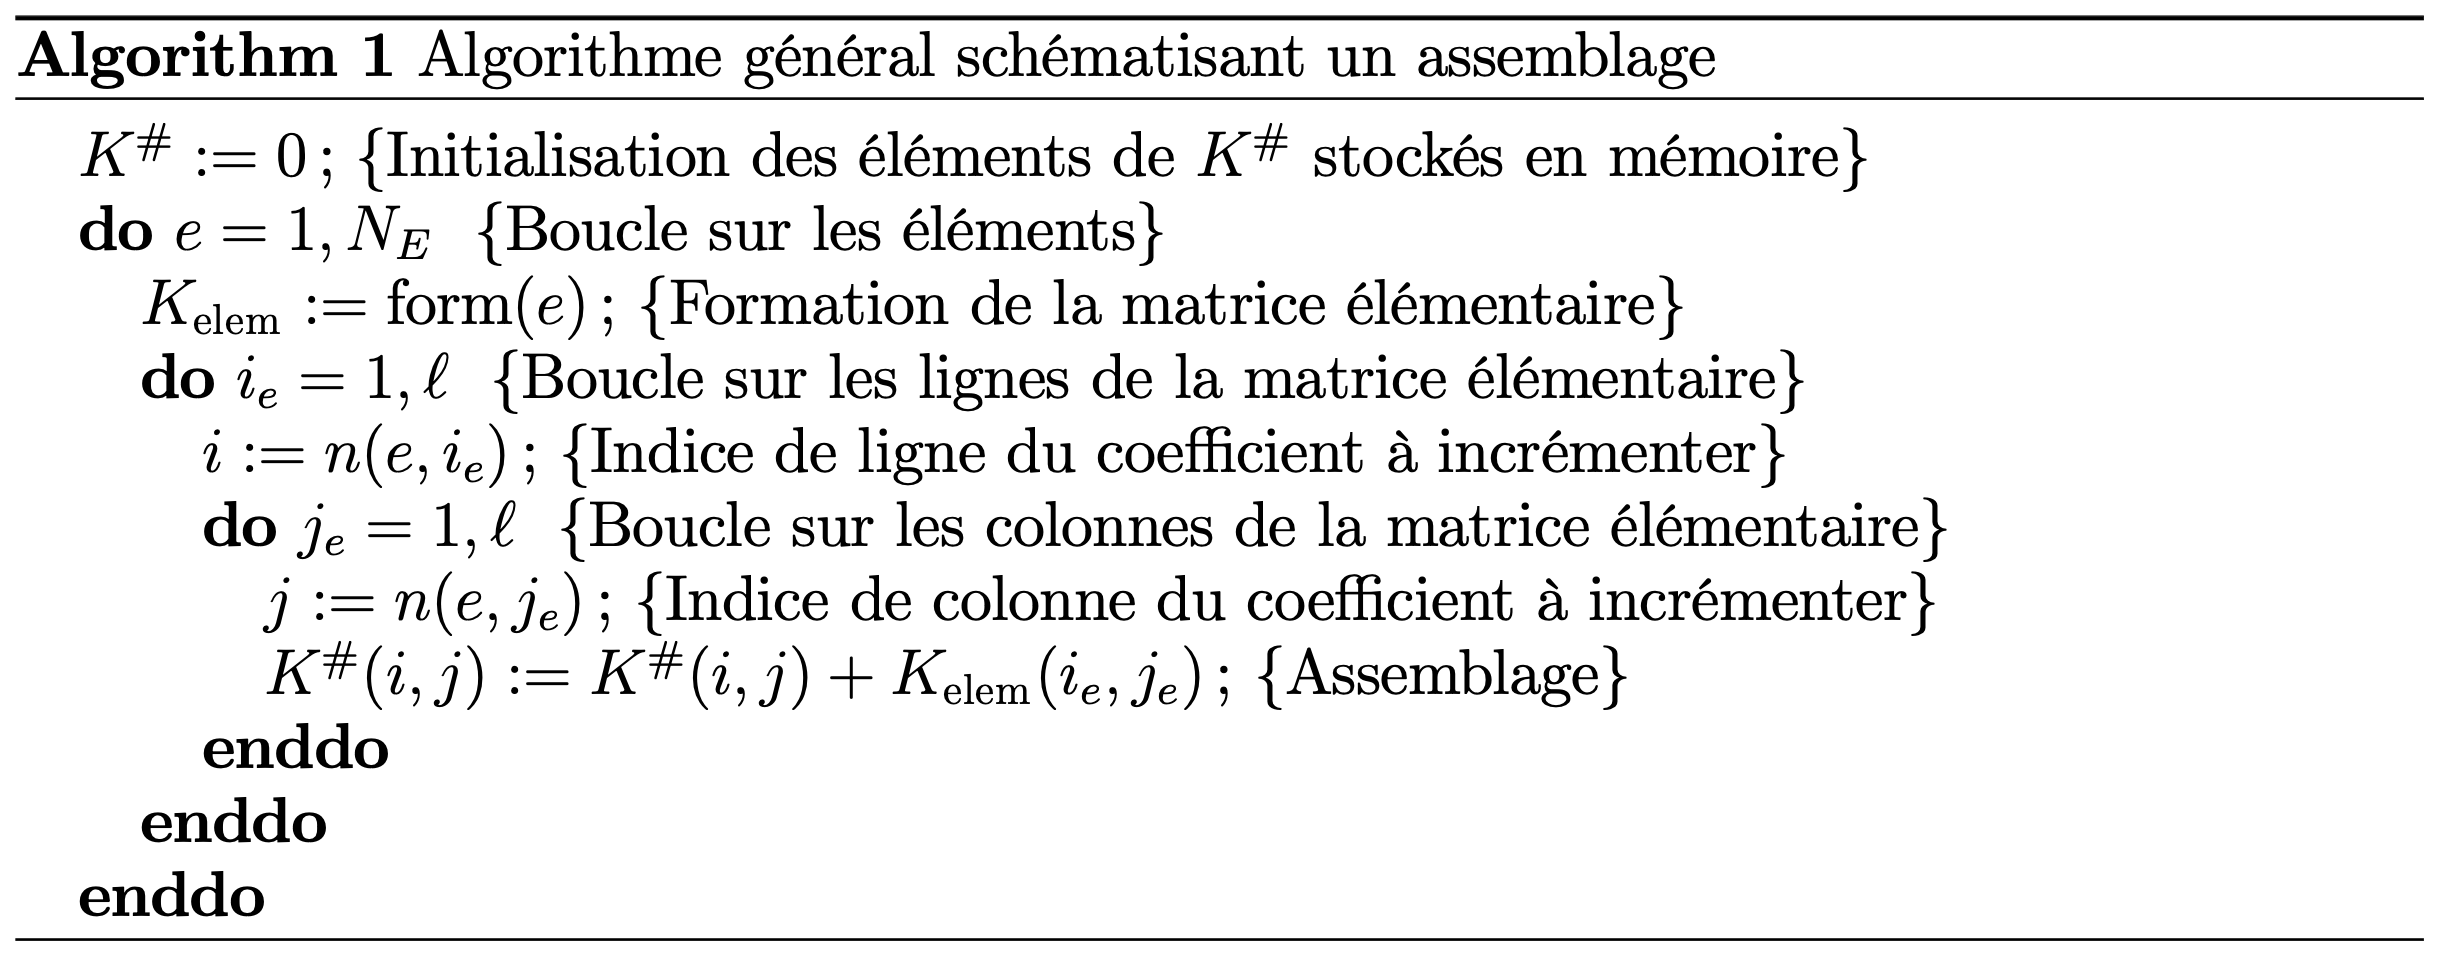
\includegraphics[scale=0.35]{algorithmeAssemblage.png} 
\end{center}
\end{frame}

%%%%%%%%%%%%%%%%%%%%%%%%%%%%%%%%%%%%%%%%%%%%%%%%%%%%%
\begin{frame}
\frametitle{Éléments finis 2D}
%Considérons le problème suivant:
\[
({\cal P}_v)\;\left\{
\begin{array}{l}
\mbox{Trouver } u\in V \mbox{ vérifiant}\\
a(u,v)=\ell(v)\quad \forall v\in V
\end{array}
\right.
\]

où \[ a(u,v)=\displaystyle \int_{\Omega}\nabla u\cdot \nabla v \quad \mbox{ et }\quad \ell(v)=\displaystyle \int_{\Omega}f v  \]
%Maillage
\begin{center}
\begin{tikzpicture}[domain=0:5,scale=1]
 \pgfmathsetmacro{\alpha}{0.05}
  \pgfmathsetmacro{\a}{1.2}
  \pgfmathsetmacro{\N}{3}
  \draw[->] (0,0) -- (\N*\a+\a/2,0)  node[right] {$x$};
  \draw[->] (0,0) -- (0,\N*\a+\a/2) node[left] {$y$};

  \foreach \n in {0,1,...,\N}{
   \draw[blue,thick](\n*\a,0)-- ++(0,\N*\a);
    \draw[blue,thick](0,\n*\a)-- ++(\N*\a,0);
}
  \foreach \n in {0,1,...,\N}{
   \draw[blue,thick](\n*\a,0)-- (\N*\a,\N*\a-\n*\a);
    \draw[blue,thick](0,\n*\a)-- (\N*\a-\n*\a,\N*\a);
}
  \foreach \i in {0,1,...,\N}{
  		\foreach \j in {0,1,...,\N}{
  		\pgfmathsetmacro{\x}{int(\N*\j+\j+\i)}
   \draw[red,thick](\i*\a,\j*\a-\a/4) node{\x};
   }
}
\pgfmathsetmacro{\M}{int(\N-1)}
  \foreach \i in {0,1,...,\M}{
  		\foreach \j in {0,1,...,\M}{
  		\pgfmathsetmacro{\x}{int(\N*\j+\j+\i)}
  		\pgfmathsetmacro{\k}{int(2*\i+2*\j*\N)}
   \draw[gray,thick](\i*\a+\a/3,\j*\a+2*\a/3) node{(\k)};
   \pgfmathsetmacro{\k}{int(2*\i+1+2*\j*\N)}
   \draw[gray,thick](\i*\a+2*\a/3,\j*\a+\a/3) node{(\k)};
   }
}



\draw (1*\a,0)  node[below] {$\scriptstyle  i h$};
\draw (0,2*\a)  node[left] {$\scriptstyle  j h$};
%\draw[fill=orange!30, fill opacity=0.6] (1*\a,2*\a)  -- ++(\a,0) -- ++(0,\a) ;
%  \path[fill=gray] (1*\a,2*\a) circle (0.6mm)node[left,below] {$\scriptstyle  a_{ij}$};
%  \draw[blue] (1.6*\a,2.2*\a) node{$\scriptstyle  K_{i,j,1}$};
%  \draw[fill=olive!30, fill opacity=0.6] (1*\a,2*\a)  -- ++(0,\a) -- ++(\a,0) ;
%  \draw[blue] (1.4*\a,2.8*\a) node{$\scriptstyle  K_{i,j,0}$};
\end{tikzpicture}
\end{center}


\end{frame}
%%%%%%%%%%%%%%%%%%%%%%%%%%%%%%%%%%%%%%%%%%%%%%%%%%%%%%%

\begin{frame}
\frametitle{Éléments finis triangles de type (1)}

\begin{center}
\begin{tikzpicture}[domain=0:5,scale=0.5]
 \pgfmathsetmacro{\alpha}{0.05}
  \pgfmathsetmacro{\a}{0.5}
  \draw[->] (0,0) -- (5,0)  node[right] {$x$};
  \draw[->] (0,0) -- (0,5) node[left] {$y$};
  \draw (3,0)  node[above right] {$\scriptstyle  \widehat{a}_1$};
  \draw (0,3)  node[above right] {$\scriptstyle  \widehat{a}_2$};
  \draw (0,0)  node[above left] {$\scriptstyle  \widehat{a}_3$};
  \draw (0.8,1.5)  node {$\scriptstyle  \widehat{x}$};
  \draw (12.2,2.4)  node {$\scriptstyle  x$};
 \draw[->] (8,0) -- ++(7,0)  node[right] {$X$};
  \draw[->] (8,0) --++ (0,5) node[left] {$Y$};
   \draw[blue,thick,fill=blue!30, fill opacity=0.6](10,2)-- ++(3,-1)-- ++(0,3)-- ++(-3,-2);

\path[fill=gray] (10,2) circle (1.0mm)node[left,below] {$\scriptstyle  a_3$};
\path[fill=gray] (13,1) circle (1.0mm)node[left,below] {$\scriptstyle  a_1$};
\path[fill=gray] (13,4) circle (1.0mm)node[right] {$\scriptstyle  a_2$};


\draw[fill=orange!30, fill opacity=0.6] (0,0) -- ++(3,0) -- ++(-3,3) -- ++(0,-3) ;

 \draw [->, >=latex,olive] (1,1.5) arc (120:70:13) ;
\end{tikzpicture}

\end{center}
\[\varphi_i = \lambda_i,\quad   1\leq i\leq 3\]
où \[\lambda_i = x_i,\quad   1\leq i\leq n\quad \mbox{ et } \lambda_{n+1}=1-\sum_{i=1}^n\lambda_i\]
\[\lambda_1=x,\quad \lambda_2=y,\quad \lambda_3=1-x-y\] 
Donc
\[\myredbox{\varphi_1=x,\quad \varphi_2=y,\quad \varphi_3=1-x-y}\] 
\end{frame}

%%%%%%%%%%%%%%%%%%%%%%%%%%%%%%%%%%%%%%%%%%%%%%%%%%%%%%%


%%%%%%%%%%%%%%%%%%%%%%%%%%%%%%%%%%%%%%%%%%%%%%%%%%%%%%%

\begin{frame}
\frametitle{Matrice élémentaire}
\begin{itemize}
\item Matrice $A=(a_{ij})_{1\leq i,j \leq 3}$ où 
\[a_{ij} = a(\varphi_i,\varphi_j)=\displaystyle \int_{\Omega}\nabla \varphi_i\cdot \nabla \varphi_j\] 
\[\nabla\varphi_1=\left(\begin{array}{c} 1\\0\end{array}\right)
 ,\quad \nabla\varphi_2=\left(\begin{array}{c} 0\\1\end{array}\right),\quad \nabla\varphi_3=\left(\begin{array}{c} -1\\-1\end{array}\right)\] 
 \[\myredbox{A=\frac 12 \left(\begin{array}{cc} 1&-1\\-1&1\end{array}\right)}\]
 \item Second membre $B=(b_i)_{1\leq i\leq 3}$ où
 \[\myredbox{b_{i} = \ell(\varphi_i)=\displaystyle \int_{\Omega} f \varphi_i}\] 
\end{itemize}
\end{frame}


%%%%%%%%%%%%%%%%%%%%%%%%%%%%%%%%%%%%%%%%%%%%%%%%%%%

\begin{frame}
\frametitle{Maillage}
\begin{itemize}
\item  Table de nœuds:
\begin{center}
\begin{tabular}{|c|c|c|c|c|c|c|c|c|c|c|c|c|c|c|c|c|c|}\hline 
{\bf n} & 0 & 1 & 2 & 3 &4 &5 &6 & 7 & 8 &9 &10 & 11  & 12 &13 &14 & 15\\ \hline 
$\mbox{\bf i} $& $0$ & $1$ & 2 & 3 & $0$ & $1$ & 2 & 3& $0$ & $1$ & 2 & 3& $0$ & $1$ & 2 & 3\\ \hline 
$\mbox{\bf j} $& $0$ & $0$ & 0 & 0 & 1 & $1$ & 1 & 1&2&2&2&2  &3&3&3&3\\ \hline 
\end{tabular}
\end{center}
\item Table de connectivité:
\begin{center}
\begin{tabular}{|c|c|c|c|c|c|c|c|c|c|c|c|c|c|c|c|c|}\hline 
{\bf e} & 0 & 1 & 2 & 3 & 4 & 5 & 6 & 7 & 8 &9  &10 & 11  & 12 &... & 17\\ \hline 
{\bf 0}& 0  & 5 & 1 & 6 & 2 & 7 & 4 & 9& 5 &10 & 6 & 11 & 8 & ... &  15\\ \hline 
{\bf 1}& 5 & 0  & 6 & 1 & 7 & 2 & 9 & 4&10&5  &11 &6   &13&... &10\\ \hline 
{\bf 2}& 4 & 1  & 5 & 2 & 6 & 3 & 8 & 5&9 &6  &10  &7   &12&... &11\\ \hline 
\end{tabular}
\end{center}
\end{itemize}




\end{frame}


%%%%%%%%%%%%%%%%%%%%%%%%%%%%%%%%%%%%%%%%%%%%%%%%%%%%%
\begin{frame}
\frametitle{Éléments finis 1D}
Considérons le problème suivant:
\[
({\cal P})\;\left\{
\begin{array}{rl}
-\displaystyle \frac{\de^2 u}{dx^2}=p&\mbox{dans } \Omega=]0,L[\\
u=0& \mbox{sur } \Gamma_1=\{0\} \\
\displaystyle \frac{\de u}{dx}=f & \mbox{sur } \Gamma_2=\{L\} 
\end{array}
\right.
\]
Formulation variationnelle: $
({\cal P}_v)\;\left\{
\begin{array}{l}
\mbox{Trouver } u\in V \mbox{ vérifiant}\\
a(u,v)=\ell(v)\quad \forall v\in V
\end{array}
\right.
$

où \[ a(u,v)=\displaystyle \int_0^L\frac{\de u}{dx}\cdot \frac{\de v}{dx}\,\de x\quad \mbox{ et }\quad \ell(v)=\displaystyle \int_0^L p\cdot v(x)\de x +f_L \cdot v(L)\]
Maillage
\begin{center}
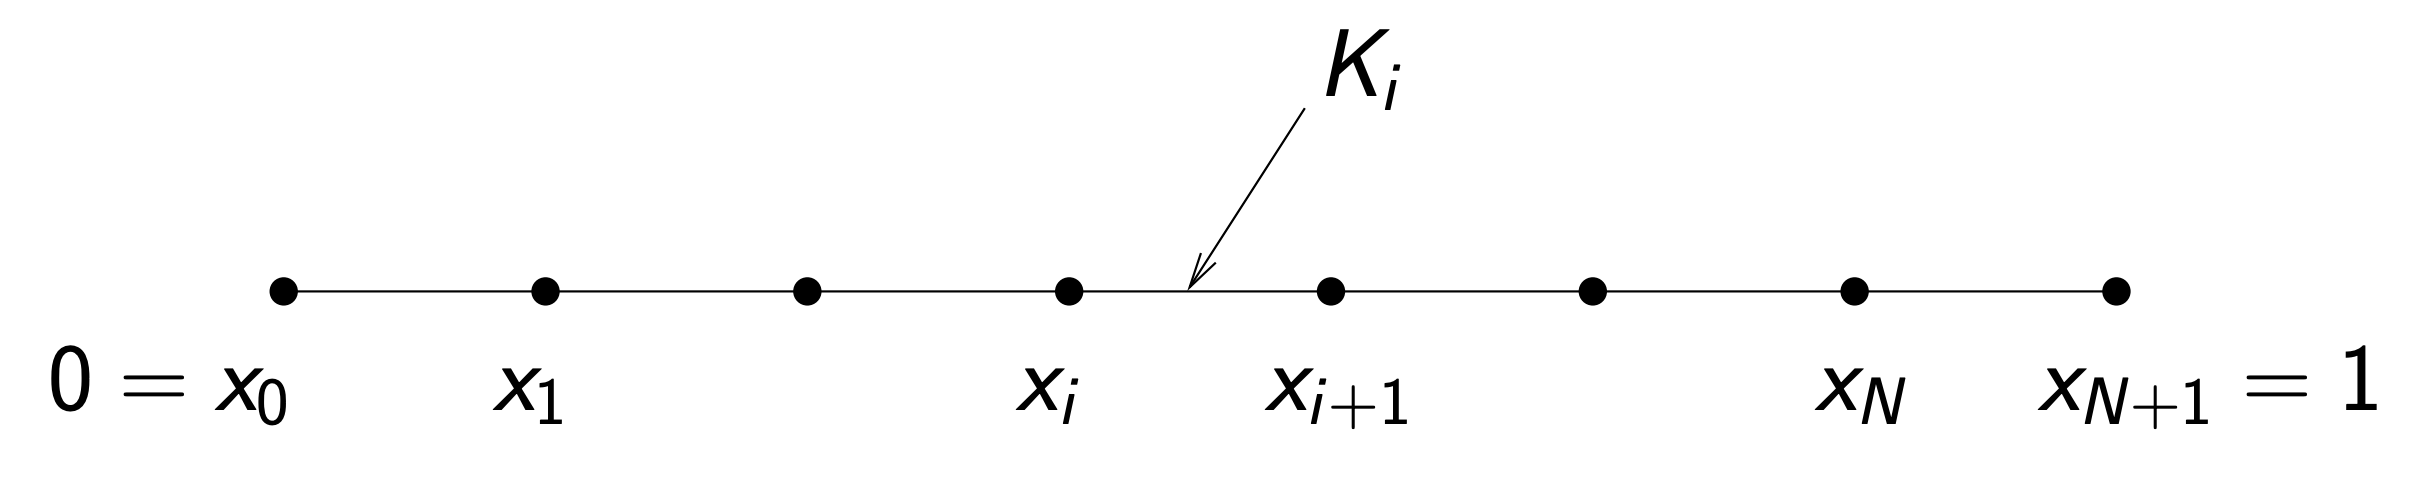
\includegraphics[scale=0.2]{mailleD1.png} 
\end{center}
\end{frame}

%%%%%%%%%%%%%%%%%%%%%%%%%%%%%%%%%%%%%%%%%%%%%%%%%%%%%
\begin{frame}
\frametitle{Eléments finis sans matrice élémentaire}
 
 \begin{center}
 \begin{tikzpicture}[domain=0:5]
  \draw[->] (-0.1,0) -- (8.5,0)  node[right] {$\scriptstyle x$};
  \draw[->] (0,-0.1) -- (0,1.5) node[above] {$\scriptstyle y$};
  \draw[olive] (0,0) --++ (1,0) --++ (1,1) --++ (1,-1)--++ (2,0)--++ (1,1) --++ (1,-1)--++ (1,0);
  \path[fill=black]  (0,0) circle (.4mm) [fill=orange] node[below] {$\scriptstyle 0=x_0$};
 \path[fill=black]  (0,0) circle (.4mm) [fill=orange];
 \path[fill=black]  (1,0) circle (.4mm) [fill=orange];
 \path[fill=black]  (2,0) circle (.4mm) [fill=orange] node[below] {$\scriptstyle x_{i}$};
  \path[fill=black]  (3,0) circle (.4mm) [fill=orange] ;
 \path[fill=black]  (3,0) circle (.4mm) [fill=orange];
   \path[fill=black]  (4,0) circle (.4mm) [fill=orange];
    \path[fill=black]  (5,0) circle (.4mm) [fill=orange] ;
    \path[fill=black]  (6,0) circle (.4mm) [fill=orange] node[below] {$\scriptstyle x_{j}$};
    \path[fill=black]  (7,0) circle (.4mm) [fill=orange] ;
    \path[fill=black]  (8,0) circle (.4mm) [fill=orange] node[below] {$\scriptstyle 1=x_{n+1}$};
\draw (2,1.2)node[above] {$\scriptstyle \varphi_i$};
\draw (6,1.2)node[above] {$\scriptstyle \varphi_j$};
\end{tikzpicture}
 \end{center}

 \begin{center}
 \begin{tikzpicture}[domain=0:5]
  \draw[->] (-0.1,0) -- (8.5,0)  node[right] {$\scriptstyle x$};
  \draw[->] (0,-0.1) -- (0,1.5) node[above] {$\scriptstyle y$};
  \draw[olive] (0,0) --++ (2,0) --++ (1,1) --++ (1,-1)--++ (4,0);
  \draw[olive] (0,0) --++ (3,0) --++ (1,1) --++ (1,-1)--++ (3,0);
  \path[fill=black]  (0,0) circle (.4mm) [fill=orange] node[below] {$\scriptstyle 0=x_0$};
 \path[fill=black]  (0,0) circle (.4mm) [fill=orange];
 \path[fill=black]  (1,0) circle (.4mm) [fill=orange];
 \path[fill=black]  (2,0) circle (.4mm) [fill=orange] ;
 \path[fill=black]  (3,0) circle (.4mm) [fill=orange]node[below] {$\scriptstyle x_{i}$};
   \path[fill=black]  (4,0) circle (.4mm) [fill=orange]node[below] {$\scriptstyle x_{j}$};
    \path[fill=black]  (5,0) circle (.4mm) [fill=orange] ;
    \path[fill=black]  (6,0) circle (.4mm) [fill=orange] ;
    \path[fill=black]  (7,0) circle (.4mm) [fill=orange] ;
    \path[fill=black]  (8,0) circle (.4mm) [fill=orange] node[below] {$\scriptstyle 1=x_{n+1}$};
\draw (3,1.2)node[above] {$\scriptstyle \varphi_i$};
\draw (4,1.2)node[above] {$\scriptstyle \varphi_j$};
\end{tikzpicture}
 \end{center}
 
 \begin{center}
 \begin{tikzpicture}[domain=0:5]
  \draw[->] (-0.1,0) -- (8.5,0)  node[right] {$\scriptstyle x$};
  \draw[->] (0,-0.1) -- (0,1.5) node[above] {$\scriptstyle y$};
   \draw[olive] (0,0) --++ (3,0) --++ (1,1) --++ (1,-1)--++ (3,0);
  \path[fill=black]  (0,0) circle (.4mm) [fill=orange] node[below] {$\scriptstyle 0=x_0$};
 \path[fill=black]  (0,0) circle (.4mm) [fill=orange];
 \path[fill=black]  (1,0) circle (.4mm) [fill=orange];
 \path[fill=black]  (2,0) circle (.4mm) [fill=orange] ;
   \path[fill=black]  (4,0) circle (.4mm) [fill=orange]node[below] {$\scriptstyle x_{i}=x_{j}$};
    \path[fill=black]  (5,0) circle (.4mm) [fill=orange] ;
    \path[fill=black]  (6,0) circle (.4mm) [fill=orange] ;
    \path[fill=black]  (7,0) circle (.4mm) [fill=orange] ;
    \path[fill=black]  (8,0) circle (.4mm) [fill=orange] node[below] {$\scriptstyle 1=x_{n+1}$};
\draw (4,1.2)node[above] {$\scriptstyle \varphi_i = \varphi_j$};
\end{tikzpicture}
 \end{center}
\end{frame}
%%%%%%%%%%%%%%%%%%%%%%%%%%%%%%%%%%%%%%%%%%%%%%%%%
\begin{frame}
%\lipsum[2]

	\begin{itemize}
  	\item \fbox{$k=1$} le segment de type (1) est obtenu pour
    \[\mathbb{P}=\mathbb{P}_1^{(1)},\quad \Sigma=\Sigma_1^{(1)} = \{a_1=1,a_2=0\}\]
Les fonctions de base sont les fonctions coordonnées barycentriques par rapport à $(a_1, a_2)$, i.e.  
\[\varphi_1 = \lambda_1=\xi,\quad   \varphi_2 = \lambda_2=1-\xi\]


  	\begin{center}
  	\begin{tabular}{cc}
  	\begin{tikzpicture}[scale=2]
\draw  [very thin, gray] [->]  (-0.2,0) -- (1.2,0); 
\draw  [very thin, gray] [->] (0,-0.2) -- (0,1.2);
\draw  [line width=1pt] (0,0) -- (1,0);
\draw  [dashed] (1,0) -- (1,1);
\node [blue] at (0,0) {$\bullet$};
\node [blue] at (1,0) {$\bullet$};
\node at (0.5,-0.5) {$\scriptstyle \varphi_1(\xi)=\xi$};
\draw [orange,domain=0:1] plot(\x,\x);
\end{tikzpicture} 
 &
 \begin{tikzpicture}[scale=2]
\draw  [very thin, gray] [->]  (-0.2,0) -- (1.2,0); 
\draw  [very thin, gray] [->] (0,-0.2) -- (0,1.2);
\draw  [line width=1pt] (0,0) -- (1,0);
\draw  [dashed] (0,0) -- (0,1);
\node [blue] at (0,0) {$\bullet$};
\node [blue] at (1,0) {$\bullet$};
\node at (0.5,-0.5) {$\scriptstyle  \varphi_2(\xi)=1-\xi$};
\draw [orange,domain=0:1] plot(\x,1-\x);

\end{tikzpicture} 
\end{tabular}
  	\end{center}
  	

  \end{itemize}	
 \end{frame}  


%%%%%%%%%%%%%%%%%%%%%%%%%%%%%%%%%%%%%%%%%%%%%%%%%%%%%
\begin{frame}
\frametitle{Construction de l'espace $V_h$}
\[a(\varphi_1,\varphi_1)=a(\varphi_1,\varphi_1)=\frac 1h\]
\[a(\varphi_1,\varphi_2)=a(\varphi_2,\varphi_1)=-\frac 1h\]
Le système élémentaire s'écrit:
\[\left(\begin{array}{r} 
f_{1}\\f_{2}
\end{array}\right)=\frac{1}{h}\left(\begin{array}{rr} 
1&-1\\-1&1
\end{array}\right) \left(\begin{array}{l} 
u_{1}\\u_{2}
\end{array}\right)
\]

\end{frame}

%%%%%%%%%%%%%%%%%%%%%%%%%%%%%%%%%%%%%%%%%%%%%%%%%%%%%
\begin{frame}
\frametitle{Assemblage en dim=1}
On choisit $n=4$, soit $(u_0,u_1,u_2,u_3,u_4)$ les déplacements aux 5 nœuds. La matrice élémentaire de l'élément $e_i$, $i=0,3$ est donnée
par
\[\left(\begin{array}{r} 
f_{i}\\f_{i+1}
\end{array}\right)=\frac{EA_i}{h_i}\left(\begin{array}{rr} 
1&-1\\-1&1
\end{array}\right) \left(\begin{array}{l} 
u_{i}\\u_{i+1}
\end{array}\right)
\]
Soit explicitement pour chacune des 4 barres:
\[\left(\begin{array}{c} 
f_{0}\\f_{1}\\f_{2}\\f_{3}\\f_{4}
\end{array}\right)=\left(\begin{array}{rrrrr} 
1&-1&0&0&0\\-1&1&0&0&0\\
0&0&0&0&0\\
0&0&0&0&0\\
0&0&0&0&0
\end{array}\right) \left(\begin{array}{l} 
u_{0}\\u_{1}\\u_{2}\\u_{3}\\u_{4}
\end{array}\right)
\]
\[\left(\begin{array}{c} 
f_{0}\\f_{1}\\f_{2}\\f_{3}\\f_{4}
\end{array}\right)=\left(\begin{array}{rrrrr} 
0&0&0&0&0\\
0&1&-1&0&0\\0&-1&1&0&0\\
0&0&0&0&0\\
0&0&0&0&0
\end{array}\right) \left(\begin{array}{l} 
u_{0}\\u_{1}\\u_{2}\\u_{3}\\u_{4}
\end{array}\right)
\]
\end{frame}

%%%%%%%%%%%%%%%%%%%%%%%%%%%%%%%%%%%%%%%%%%%%%%%%%%%%%
\begin{frame}
\frametitle{Assemblage en dim=1}
\[\left(\begin{array}{c} 
f_{0}\\f_{1}\\f_{2}\\f_{3}\\f_{4}
\end{array}\right)=\left(\begin{array}{rrrrr} 
0&0&0&0&0\\
0&0&0&0&0\\
0&0&1&-1&0\\0&0&-1&1&0\\
0&0&0&0&0\\

\end{array}\right) \left(\begin{array}{l} 
u_{0}\\u_{1}\\u_{2}\\u_{3}\\u_{4}
\end{array}\right)
\]
\[\left(\begin{array}{c} 
f_{0}\\f_{1}\\f_{2}\\f_{3}\\f_{4}
\end{array}\right)=\left(\begin{array}{rrrrr} 
0&0&0&0&0\\
0&0&0&0&0\\
0&0&0&0&0\\
0&0&0&1&-1\\0&0&0&-1&1
\end{array}\right) \left(\begin{array}{l} 
u_{0}\\u_{1}\\u_{2}\\u_{3}\\u_{4}
\end{array}\right)
\]
\end{frame}

%%%%%%%%%%%%%%%%%%%%%%%%%%%%%%%%%%%%%%%%%%%%%%%%%%%%%
\begin{frame}
\frametitle{Assemblage en dim=1}
La matrice d'assemblage s'obtient en sommant les 4 matrices élémentaires:
\[\left(\begin{array}{c} 
f_{0}\\f_{1}\\f_{2}\\f_{3}\\f_{4}
\end{array}\right)=\left(\begin{array}{ccccc} 
1&-1&0&0&0\\-1&2&-1&0&0\\
0&-1&2&-1&0\\0&0&-1&2&-1\\
0&0&0&-1&1
\end{array}\right) \left(\begin{array}{l} 
u_{0}=0\\u_{1}\\u_{2}\\u_{3}\\u_{4}
\end{array}\right)
\]
On $\delta_0=0$, La première ligne nous donne la réaction à l'origine $f_0=-\frac{EA_0}{h_0}\delta_1$. Le système n'a que 4 inconnues, on obtient le système d'ordre 4 en supprimant la première ligne et la première colonne:
\[\left(\begin{array}{c} 
f_{1}\\f_{2}\\f_{3}\\f_{4}
\end{array}\right)=\left(\begin{array}{cccc} 
2&-1&0&0\\
-1&2&-1&0\\
0&-1&2&-1\\
0&0&-1&1
\end{array}\right) \left(\begin{array}{l} 
u_{1}\\u_{2}\\u_{3}\\u_{4}
\end{array}\right)
\]

\end{frame}
%%%%%%%%%%%%%%%%%%%%%%%%%%%%%%%%%%%%%%%%%%%%%%%%%%%%%
\begin{frame}
\frametitle{Code python}
\begin{center}
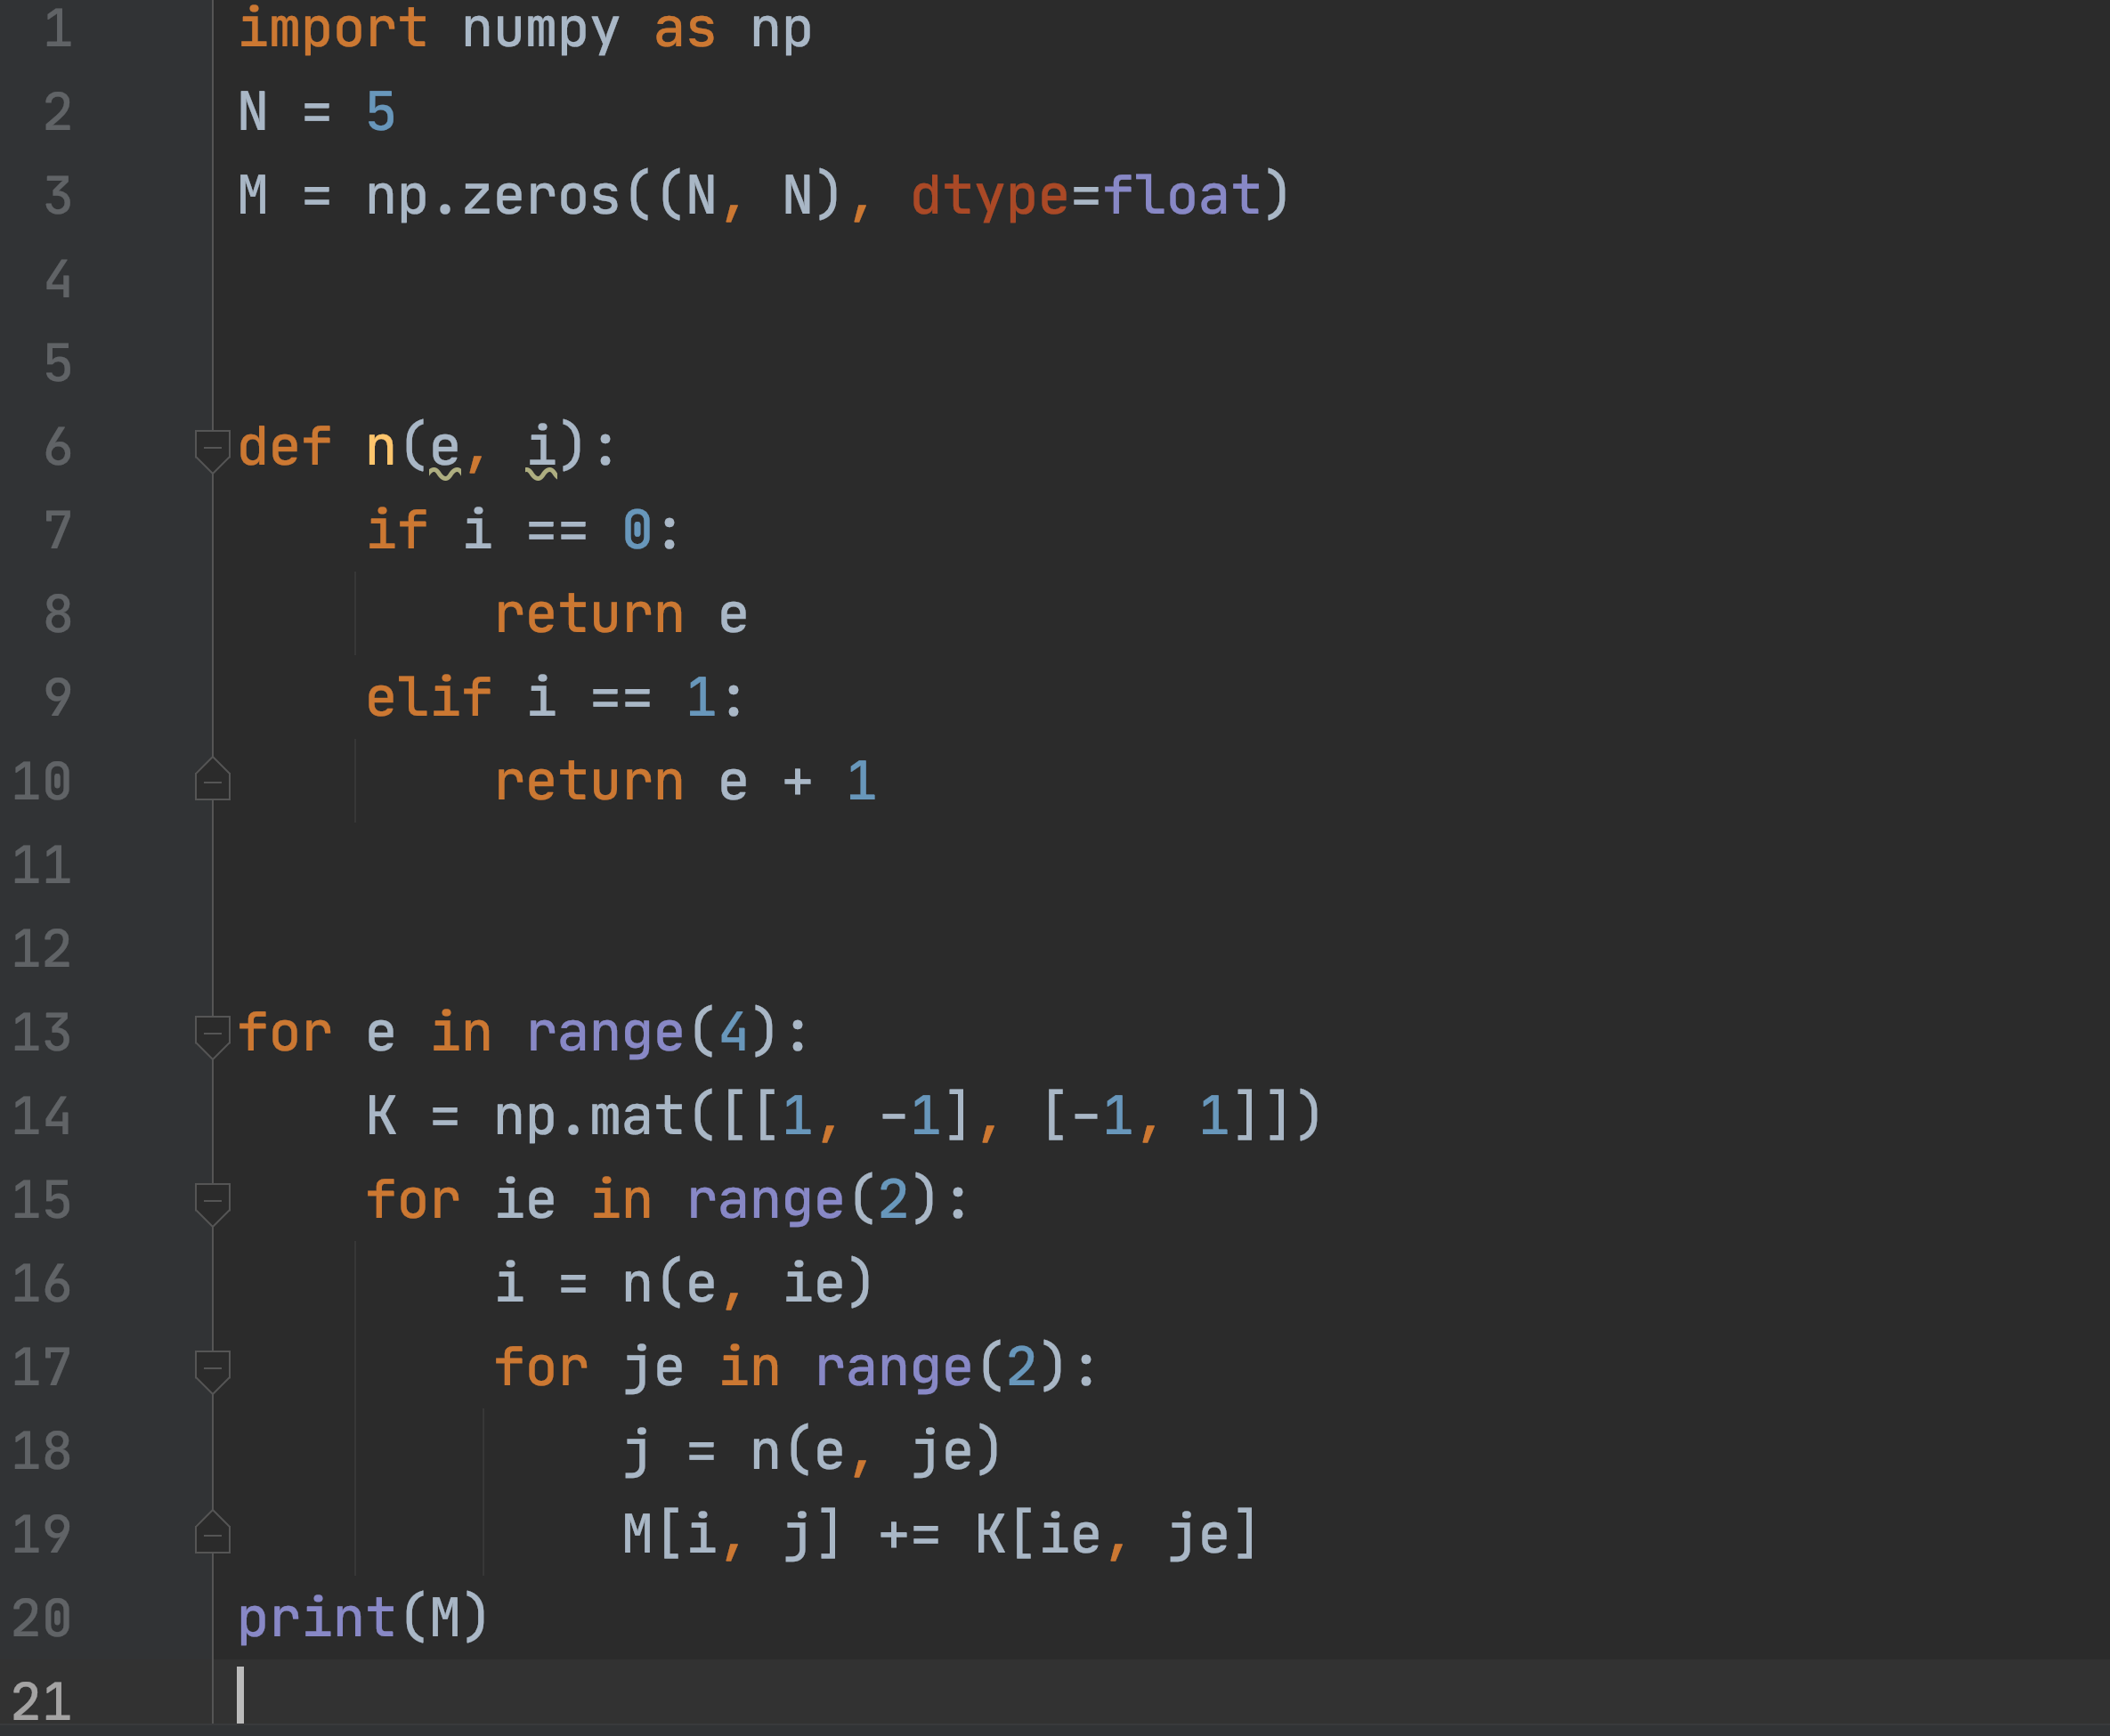
\includegraphics[scale=0.24]{codePython01.png} 
\end{center}

\end{frame}
%%%%%%%%%%%%%%%%%%%%%%%%%%%%%%%%%%%%%%%%%%%%%%%%%%%%%
\begin{frame}
\frametitle{Code python}
\begin{center}
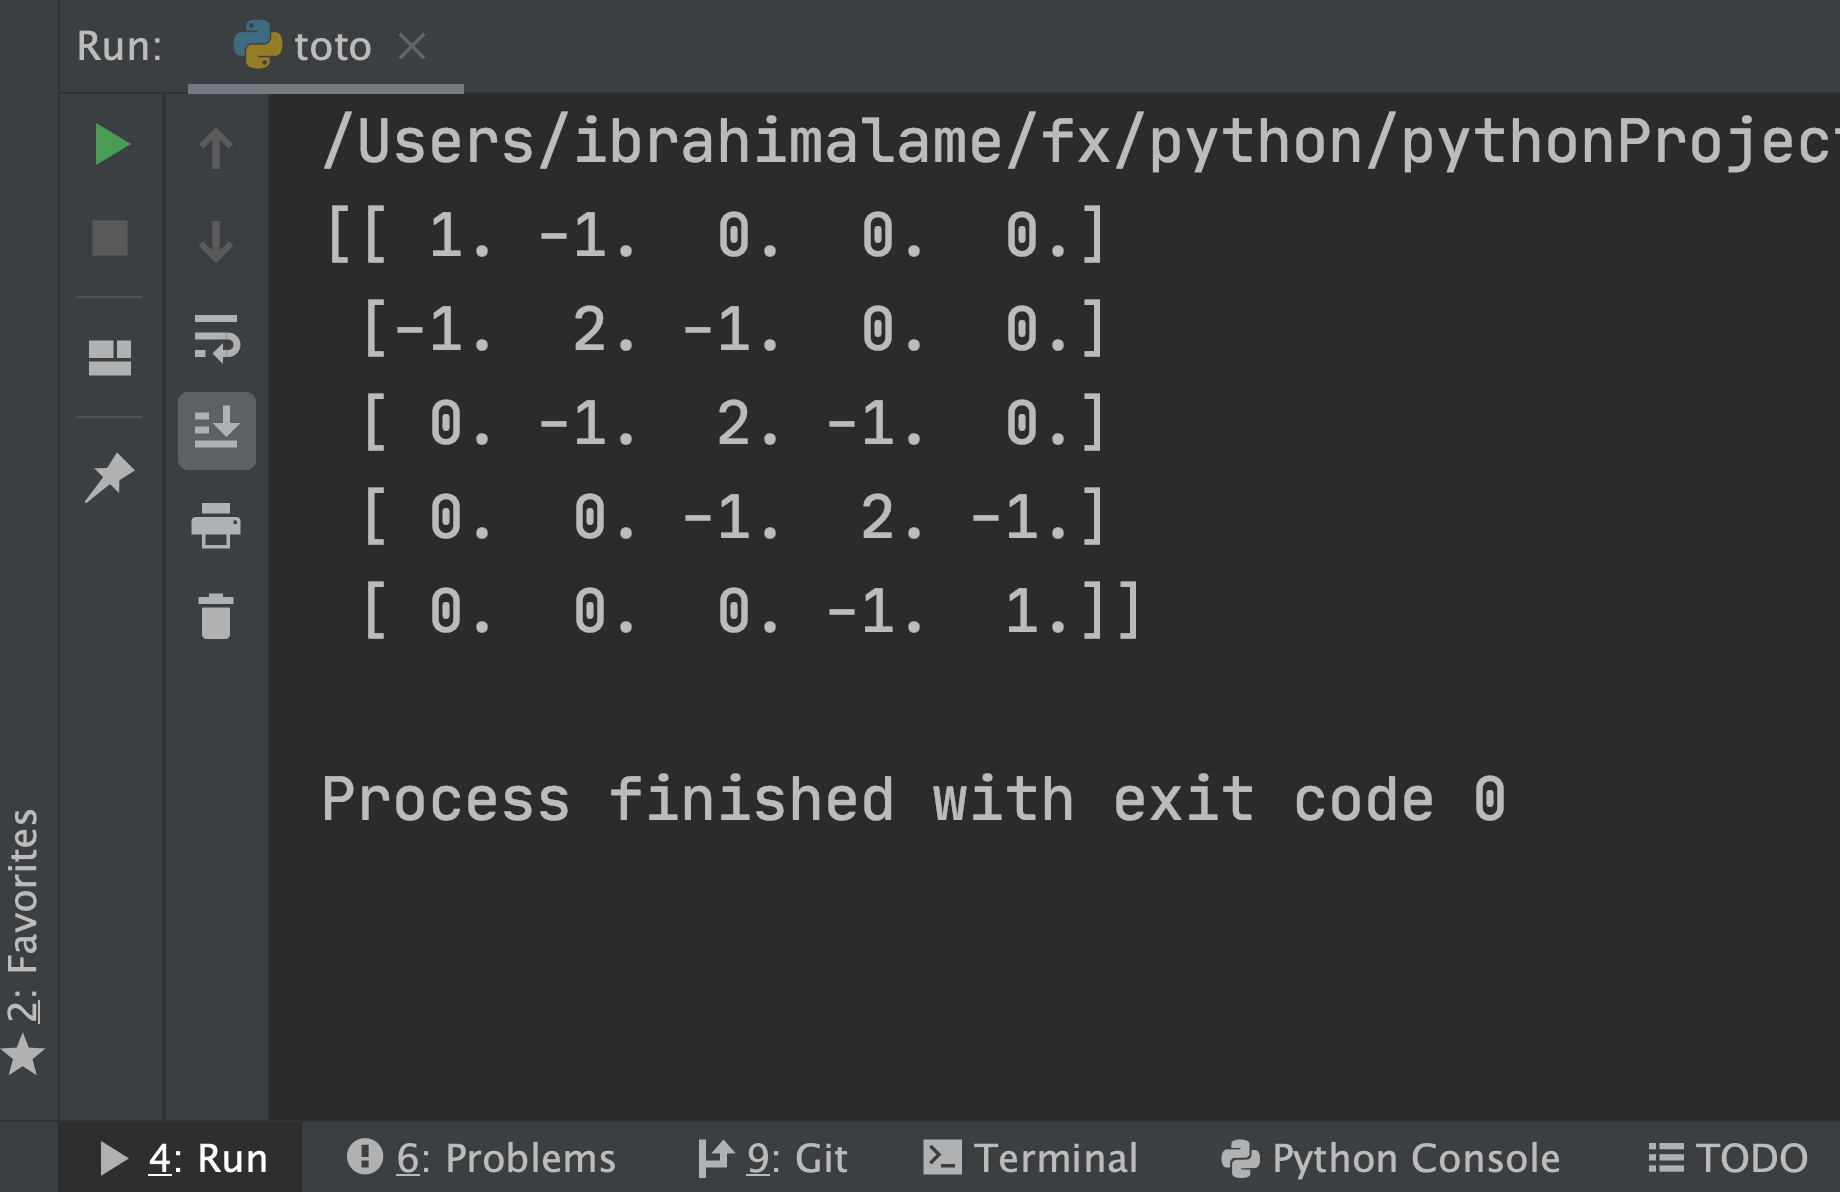
\includegraphics[scale=0.34]{codePython02.png} 
\end{center}

\end{frame}
%%%%%%%%%%%%%%%%%%%%%%%%%%%%%%%%%%%%%%%%%%%%%%%%%%%%%
\begin{frame}
\frametitle{Code python}
\begin{center}
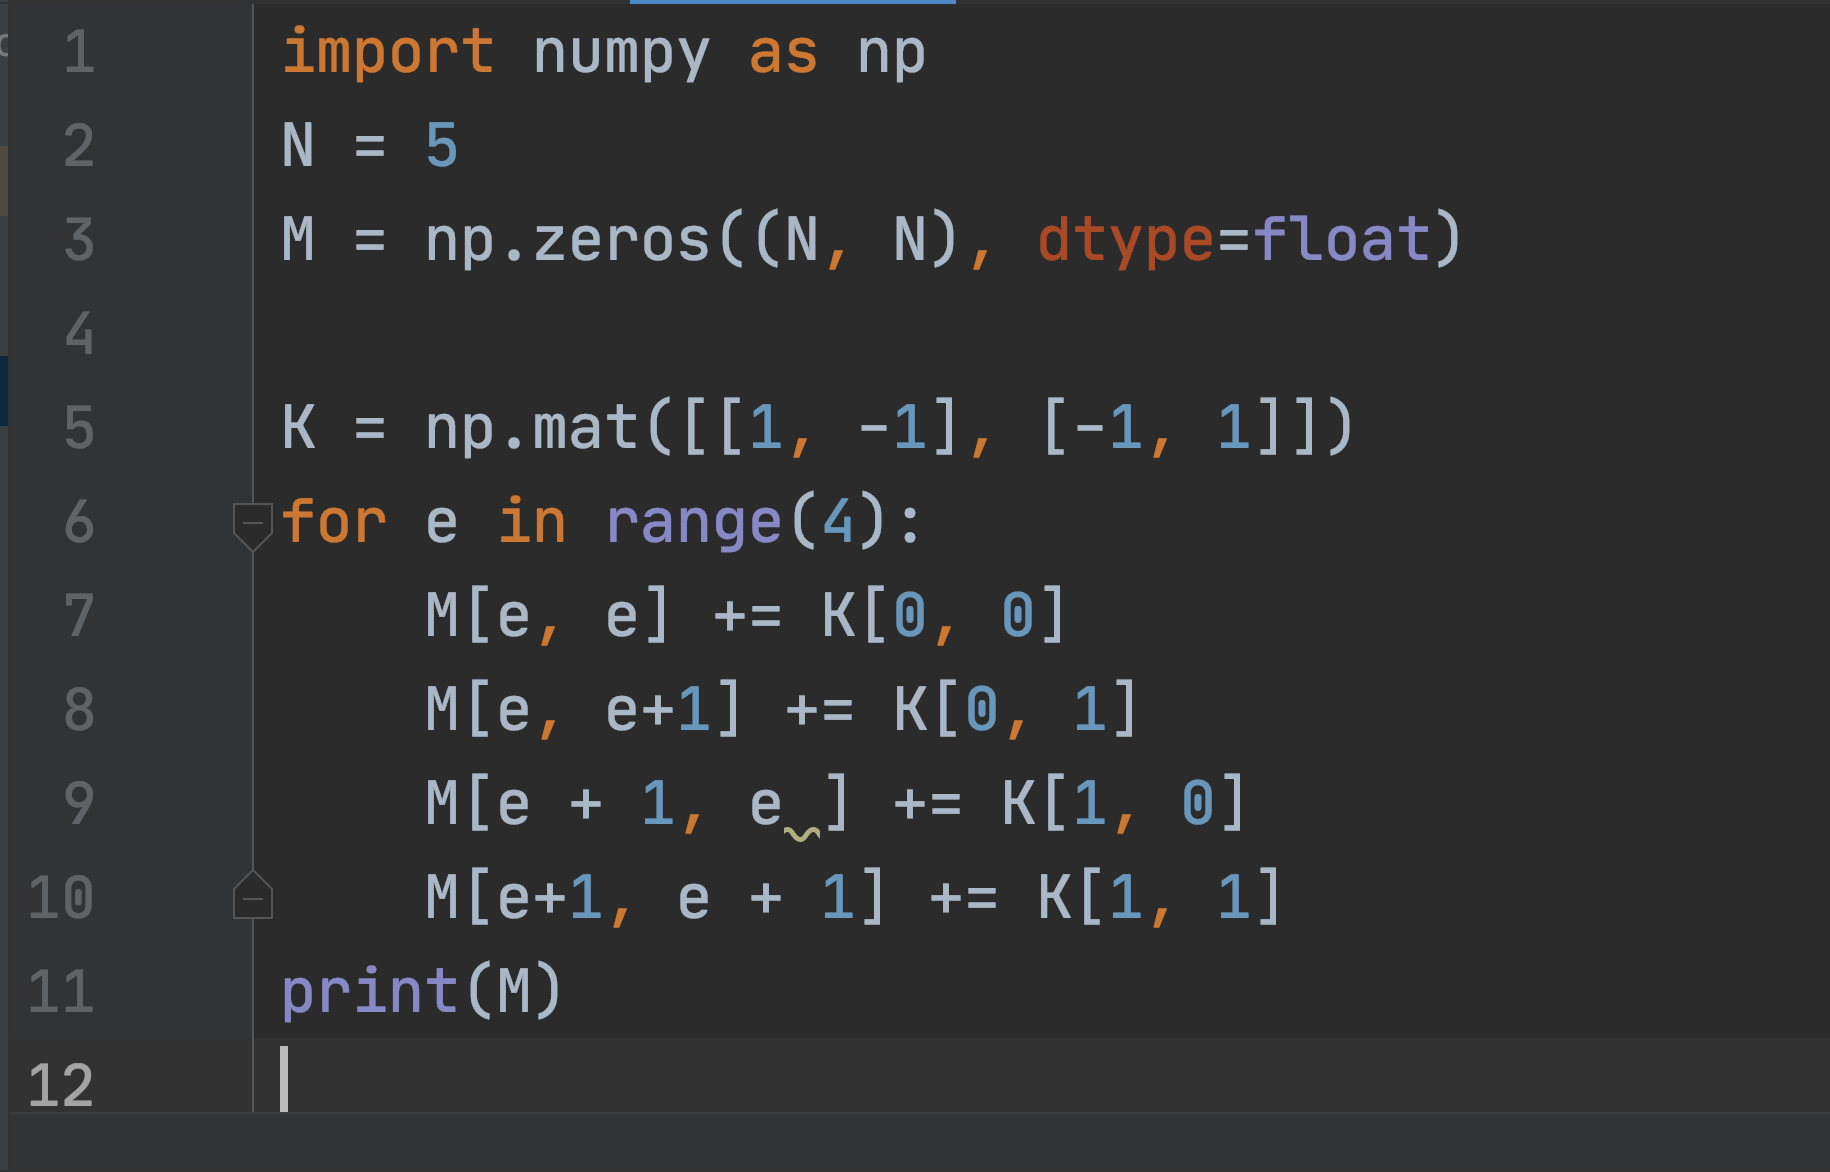
\includegraphics[scale=0.34]{codePython03.png} 
\end{center}

\end{frame}
%%%%%%%%%%%%%%%%%%%%%%%%%%%%%%%%%%%%%%%%%%%%%%%%%%%%%
\begin{frame}
\frametitle{Treillis soumis à une force nodale}
 trois poutres de même nature et de même section droite.
\begin{itemize}
\item Le noeud 1 est articulé et le nœud 3 repose sur un appui simple dont la normale est horizontale.
\item Le noeud 2 porte une charge de composantes (0, P ).
\end{itemize}
 \begin{center}
 \begin{tikzpicture}[scale=0.7]
\draw  [very thin, gray] [->]  (-2.5,0) -- (4,0); 
\draw  [very thin, gray] [->] (0,-6) -- (0,2);
\draw [double distance = 3pt] (0,0) -- (3,0) -- (0,-3*1.732) -- (0,0);
\path[fill=black]  (0,0) circle (2mm) [fill=gray];
\path[fill=black]  (3,0) circle (2mm) [fill=gray];
\path[fill=black]  (0,-3*1.732) circle (2mm) [fill=gray];
\draw [red,->,very thick] (3,0)-- (3,-2) node[right,midway]{$\vec{f_3}=\vec{P}$};
\draw [blue,->,very thick] (0,0)-- (-1.5,0) node[below,midway]{$\vec{f_0}$};
\draw [blue,->,very thick] (0,0)-- (0,1.5) node[right,midway]{$\vec{f_1}$};
\draw [blue,->,very thick] (0,-3*1.732)-- (1.2,-3*1.732) node[below,midway]{$\vec{f_4}$};
\draw (4,0) node[right] {$X$};
\draw (0,2) node[right] {$Y$};
%\draw [domain=0:5][line width=1] plot(\x,{.8598e-1*\x*\x*\x-.8104*\x*\x+1.697*\x});
%\draw [domain=0:6] plot(\x,{sin(57.29*\x)});
\end{tikzpicture} 

\end{center}


\end{frame}

%%%%%%%%%%%%%%%%%%%%%%%%%%%%%%%%%%%%%%%%%%%%%%%%%%%%%
\begin{frame}
\frametitle{Treillis soumis à une force nodale}
Le système élémentaire s'écrit:
\[\left(\begin{array}{r} 
f_{1}\\f_{2}
\end{array}\right)=\frac{1}{h}\left(\begin{array}{rr} 
1&-1\\-1&1
\end{array}\right) \left(\begin{array}{l} 
u_{1}\\u_{2}
\end{array}\right)
\]

\begin{center}
 \begin{tikzpicture}[scale=1]
\draw  [very thin, gray] [->]  (-0.2,0) -- (4,0); 
\draw  [very thin, gray] [->] (0,-0.2) -- (0,3);
\draw  [dashed] (1,0) -- (1,.5)--(0,.5);
\draw  [dashed] (3,0) -- (3,2.5)--(0,2.5);
\draw (1,0) node[below] {$X_i$};
\draw (3,0) node[below] {$X_j$};
\draw (-0.2,0.5) node[below] {$Y_i$};
\draw (-0.2,2.5) node[below] {$Y_j$};
\draw [double distance = 3pt] (1,0.5) -- (3,2.5);
\path[fill=black]  (1,.5) circle (1.2mm) [fill=gray];
\path[fill=black]  (3,2.5) circle (1.2mm) [fill=gray];
\coordinate (A) at (2,.5);
\draw[->,red] (A)  arc(0:45:1);
\draw[red] (2,.9) node[right]{$\theta$};
\draw  [dotted] (1,.5) -- (3,.5);
\draw  [very thin, gray] [->]  (0.8,0.3) -- (3.5,3.); 
\draw  [very thin, gray] [->] (1.2,0.3) -- (-1,2.5);
\draw (4,0) node[right] {$X$};
\draw (0,3.2) node[right] {$Y$};
\draw (3.5,3) node[right] {$x$};
\draw (-1,2.8) node[right] {$y$};
%\draw [domain=0:5][line width=1] plot(\x,{.8598e-1*\x*\x*\x-.8104*\x*\x+1.697*\x});
%\draw [domain=0:6] plot(\x,{sin(57.29*\x)});
\end{tikzpicture} 
\end{center}
\end{frame}

%%%%%%%%%%%%%%%%%%%%%%%%%%%%%%%%%%%%%%%%%%%%%%%%%%%%%
\begin{frame}
\frametitle{Formules de passage}
Les formules de passage entre les deux repères local $(x,y)$ et global $(X,Y)$:
\[\left(\begin{array}{l} 
u_{1}\\u_{2}
\end{array}\right) = \left(\begin{array}{cccc} 
\cos\theta &\sin\theta&0&0\\
0&0&\cos\theta &\sin\theta
\end{array}\right) \left(\begin{array}{l} 
U_{1}^x\\U_{1}^y\\U_{2}^x\\U_{2}^y
\end{array}\right)  \]
\[\left(\begin{array}{l} 
F_{1}^x\\F_{1}^y\\F_{2}^x\\F_{2}^y
\end{array}\right)   = \left(\begin{array}{cc} 
\cos\theta &0\\
\sin\theta& 0\\
0&\cos\theta \\
0 &\sin\theta
\end{array}\right)  \left(\begin{array}{l} 
f_{1}\\f_{2}
\end{array}\right)  \]


\end{frame}

%%%%%%%%%%%%%%%%%%%%%%%%%%%%%%%%%%%%%%%%%%%%%%%%%%%%%
\begin{frame}
\frametitle{Matrice de rigidité élémentaire dans le repère global}
\[\left(\begin{array}{l} 
F_{1}^x\\F_{1}^y\\F_{2}^x\\F_{2}^y
\end{array}\right)   = \frac{1}{L}\left(\begin{array}{rrrr} 
C^2&CS&-C^2&-CS\\
CS&S^2&-CS&-S^2\\
-C^2&-CS&C^2&CS\\
-CS&-S^2&CS&S^2
\end{array}\right)\left(\begin{array}{l} 
U_{1}^x\\U_{1}^y\\U_{2}^x\\U_{2}^y
\end{array}\right)  \]
Changement de notations !
\[\left(\begin{array}{l} 
f_{1}\\f_{2}\\f_{3}\\f_{4}
\end{array}\right)   = \frac{EA}{L}\left(\begin{array}{rrrr} 
C^2&CS&-C^2&-CS\\
CS&S^2&-CS&-S^2\\
-C^2&-CS&C^2&CS\\
-CS&-S^2&CS&S^2
\end{array}\right)\left(\begin{array}{l} 
\delta_{1}\\\delta_{2}\\\delta_{3}\\\delta_{4}
\end{array}\right)  \]
\end{frame}

%%%%%%%%%%%%%%%%%%%%%%%%%%%%%%%%%%%%%%%%%%%%%%%%%%%%%
\begin{frame}
\frametitle{Nœuds et connectivité}
Les caractéristique géométriques du système se résume en:\\
\begin{center}
\begin{tabular}{|l|c|r|}
  \hline
  nœud & $x$  & $y$ \\
  \hline
  0 & 0 & 0 \\
  1& $L$& 0 \\
  2& 0 & $-\sqrt 3 L$ \\
  \hline
\end{tabular} 
\end{center}

\begin{center}
  \begin{tabular}{|l|c|r|c|c|}
  \hline
  poutre & $\ell$  & $\theta$ & $C=\cos\theta$ & $S=\sin\theta$\\
  \hline
  (0,1) & $L$ & 0 & 1 & 0 \\
  (1,2)& $2L$& $-\frac{2\pi}{3}$&$-1/2$&$-\sqrt 3/2 $\\
  (2,0)& $\sqrt 3L$ &$\frac{\pi}{2}$ &0 &1 \\
  \hline
\end{tabular}
\end{center}

\end{frame}


%%%%%%%%%%%%%%%%%%%%%%%%%%%%%%%%%%%%%%%%%%%%%%%%%%%%%
\begin{frame}
\frametitle{Les systèmes élémentaires}
Écrivons l'équation d'équilibre pour chaque barre:
\[ \left(\begin{array}{r}f_0\\ f_1\\f_2\\f_3 \end{array}\right) 
 =\frac{EA}{L}\left(\begin{array}{rrrr} 
1&0&-1&0\\
0&0&0&0\\
-1&0&1&0\\
0&0&0&0
\end{array}\right)\times
\left(\begin{array}{r} \delta_0\\\delta_1\\\delta_2\\\delta_3 \end{array}\right) 
\]
\[
\left(\begin{array}{r}f_2\\ f_3\\f_4\\f_5 \end{array}\right) 
=\frac{EA}{8L}\left(\begin{array}{rrrr} 
1&\sqrt 3&-1&-\sqrt 3\\
\sqrt 3&3&-\sqrt 3&-3\\
-1&-\sqrt 3&1&\sqrt 3\\
-\sqrt 3&-3&\sqrt 3&3\\
\end{array}\right)\times
\left(\begin{array}{r} \delta_2\\ \delta_3\\\delta_4\\\delta_5 \end{array}\right) 
\]
\[\left(\begin{array}{r}f_4\\ f_5\\f_0\\f_1 \end{array}\right) 
=\frac{EA}{\sqrt 3L}\left(\begin{array}{rrrr} 
0&0&0&0\\
0&1&0&-1\\
0&0&0&0\\
0&-1&0&1
\end{array}\right)\times
\left(\begin{array}{r} \delta_4\\ \delta_5\\\delta_0\\\delta_1  \end{array}\right) 
\]
\end{frame}

%%%%%%%%%%%%%%%%%%%%%%%%%%%%%%%%%%%%%%%%%%%%%%%%%%%%%
\begin{frame}
\frametitle{Les systèmes élémentaires dans la base globale}
Ensuite, nous écrivons les trois systèmes en base 6 en fonction d'une même inconnue $(\delta_0,\delta_1,\delta_2,\delta_3,\delta_4,\delta_5)^t$ :

\[\left(\begin{array}{r}f_0\\ f_1\\f_2\\f_3\\f_4\\f_5 \end{array}\right) 
=\frac{EA}{L}
\left(\begin{array}{rrrrcc} 
1&0&-1&0&0&0\\
0&0&0&0&0&0\\
-1&0&1&0&0&0\\
0&0&0&0&0&0\\
0&0&0&0&0&0\\
0&0&0&0&0&0
\end{array}\right)\times
\left(\begin{array}{r} \delta_0\\ \delta_1\\ \delta_2\\ \delta_3\\ \delta_4\\ \delta_5  \end{array}\right) 
\]

\[\left(\begin{array}{r}f_0\\ f_1\\f_2\\f_3\\f_4\\f_5 \end{array}\right) 
=\frac{EA}{L}
\left(\begin{array}{ccrrrr} 
0&0&0&0&0&0\\
0&0&0&0&0&0\\
0&0&\frac 18&\frac{\sqrt 3}{8}&-\frac 18&-\frac{\sqrt 3}{8}\\
0&0&\frac{\sqrt 3}{8}&\frac 38&-\frac{\sqrt 3}{8}&-\frac 38\\
0&0&-\frac 18&-\frac{\sqrt 3}{8}&\frac 18&\frac{\sqrt 3}{8}\\
0&0&-\frac{\sqrt 3}{8}&-\frac 38&\frac{\sqrt 3}{8}&\frac 38\\
\end{array}\right)
\times
\left(\begin{array}{r} \delta_0\\ \delta_1\\ \delta_2\\ \delta_3\\ \delta_4\\ \delta_5   \end{array}\right)
\]
\end{frame}

%%%%%%%%%%%%%%%%%%%%%%%%%%%%%%%%%%%%%%%%%%%%%%%%%%%%%
\begin{frame}
\frametitle{Les systèmes élémentaires dans la base globale}
\[\left(\begin{array}{r}f_0\\ f_1\\f_2\\f_3\\f_4\\f_5 \end{array}\right) 
=\frac{EA}{L} \left(\begin{array}{rrccrr} 
0&0&0&0&0&0\\
0&\frac{1}{\sqrt 3}&0&0&0&-\frac{1}{\sqrt 3}\\
0&0&0&0&0&0\\
0&0&0&0&0&0\\
0&0&0&0&0&0\\
0&-\frac{1}{\sqrt 3}&0&0&0&\frac{1}{\sqrt 3}
\end{array}\right)
\times
\left(\begin{array}{r}  \delta_0\\ \delta_1\\ \delta_2\\ \delta_3\\ \delta_4\\ \delta_5   \end{array}\right)
\]
\end{frame}

%%%%%%%%%%%%%%%%%%%%%%%%%%%%%%%%%%%%%%%%%%%%%%%%%%%%%
\begin{frame}
\frametitle{Matrice d'assemblage}
\[\left(\begin{array}{r}f_0\\ f_1\\f_2\\f_3\\f_4\\f_5 \end{array}\right) 
 =\frac{EA}{L}\left(\begin{array}{rrccrr} 
1&0&-1&0&0&0\\
0&\frac{1}{\sqrt 3}&0&0&0&-\frac{1}{\sqrt 3}\\
-1&0&1+\frac 18&\frac{\sqrt 3}{8}&-\frac 18&-\frac{\sqrt 3}{8}\\
0&0&\frac{\sqrt 3}{8}&\frac 38&-\frac{\sqrt 3}{8}&-\frac 38\\
0&0&-\frac 18&-\frac{\sqrt 3}{8}&\frac 18&\frac{\sqrt 3}{8}\\
0&-\frac{1}{\sqrt 3}&-\frac{\sqrt 3}{8}&-\frac 38&\frac{\sqrt 3}{8}&\frac{ 3}{8}+\frac{1}{\sqrt 3}
\end{array}\right)
\times
\left(\begin{array}{l}  \delta_0=0\\ \delta_1=0\\ \delta_2\\ \delta_3\\ \delta_4=0\\ \delta_5   \end{array}\right)
\]
Les trois déplacements nuls $\delta_0=\delta_1=\delta_4=0$ nous permettent de réduire le système et de supprimer de la matrice globale les trois lignes 0,1,4 et les trois colonnes 0,1,4. D'où le système linéaire:

\[\myredbox{
\left(\begin{array}{r} 0\\P\\0 \end{array}\right) 
=
\frac{EA}{L}\left(\begin{array}{rrr} 
1+\frac 18&\frac{\sqrt 3}{8}&-\frac{\sqrt 3}{8}\\
\frac{\sqrt 3}{8}&\frac 38&-\frac 38\\
-\frac{\sqrt 3}{8}&-\frac 38&\frac{ 3}{8}+\frac{1}{\sqrt 3}
\end{array}\right)
\times
\left(\begin{array}{r}   \delta_2\\ \delta_3\\ \delta_5  \end{array}\right) }
\]
\end{frame}

%%%%%%%%%%%%%%%%%%%%%%%%%%%%%%%%%%%%%%%%%%%%%%%%%%%%%
\begin{frame}
\frametitle{Résolution du système}
Après avoir résolu le système linéaire réduit, on reprend les équations éliminées du système globale pour déterminer les réactions aux appuis:
\[\begin{array}{l}
f_0=-\frac{EA}{L}\delta_2\\
f_1=-\frac{EA}{L}\frac{1}{\sqrt 3}\delta_5\\
f_4=\frac{EA}{L}\left(-\frac{\sqrt 3}{8} \delta_2-\frac{ 3}{8}\delta_3  +(\frac{ 3}{8}+\frac{1}{\sqrt 3})\delta_5\right)
\end{array}
\]
 On trouve $\delta_2\simeq 0.06$mm,  $\delta_3\simeq-0.47$mm,  $\delta_5\simeq-0.17$mm.\\
 et $f_0\simeq -5.8\times 10^3$N,  $f_1\simeq 1.0\times 10^4$N, $f_4\simeq 5.8\times 10^3$N.
 \begin{center}
 \begin{tikzpicture}[scale=0.6]
\draw  [very thin, gray] [->]  (-1,0) -- (4,0); 
\draw  [very thin, gray] [->] (0,-6) -- (0,0.5);
\draw [double distance = 3pt] (0,0) -- (3,0) -- (0,-3*1.732) -- (0,0);
\draw [blue,double distance = 3pt] (0,0) -- (3.06,-0.47) -- (0,-3*1.732-0.17) -- (0,0);
\draw [red,->,very thick] (3.06,-0.47)-- (3.06,-0.47-2);
\path[fill=black]  (0,0) circle (2mm) [fill=gray];
\path[fill=black]  (3,0) circle (2mm) [fill=gray];
\path[fill=black]  (0,-3*1.732) circle (2mm) [fill=gray];
\path[blue,fill=black]  (3.06,-0.47) circle (2mm) [fill=blue];
\path[blue,fill=black]  (0,-3*1.732-0.17) circle (2mm) [fill=blue];

\draw (4,0) node[right] {$X$};
\draw (0,0.5) node[right] {$Y$};
%\draw [domain=0:5][line width=1] plot(\x,{.8598e-1*\x*\x*\x-.8104*\x*\x+1.697*\x});
%\draw [domain=0:6] plot(\x,{sin(57.29*\x)});
\end{tikzpicture} 

\end{center}


\end{frame}

%%%%%%%%%%%%%%%%%%%%%%%%%%%%%%%%%%%%%%%%%%%%%%%%%%%%%
\begin{frame}[fragile]
\frametitle{Mise en œuvre numérique}

{\large Géométrie du problème}

\[Points=\left([x_i,y_i]\right)_{i=0,n-1}\]
\[Barres=\left([p_i,p_j]\right)_{(i,j)\in G}\]
 En python $N$ et $B$ sont codés par les deux listes suivantes:
\begin{verbatim}
L = .7
Points = [[0, 0], [0, L], [L, 0]]
Barres = [[0, 1], [1, 2], [2, 0]]
\end{verbatim}
Un nœud peut être articulé en un point fixe qui empêche tout déplacement  $u_1=u_2=0$, ou un appui simple horizontal ($u_2=0$) ou vertical ($u_1=0$). On représente la fixation d'un nœud par un triplet $\left(p_i,\alpha_i,\beta_i\right)$ où $p_i$ est le point considéré, $\alpha_i$ est un boolean qui vaut 1 si le déplacement horizontal est libre, 0 sinon, et $\beta_i$ est un boolean qui vaut 1 si le déplacement vertical est libre, 0 sinon. Pour notre exemple:
\begin{verbatim}
Conditions = [[0,0,0],[2,0,1]]
\end{verbatim}
\end{frame}

%%%%%%%%%%%%%%%%%%%%%%%%%%%%%%%%%%%%%%%%%%%%%%%%%%%%%
\begin{frame}[fragile]
\frametitle{Mise en œuvre numérique}
{\Large Les constantes et grandeurs physiques}

La section des barres $A$ exprimée en $\mbox{m}^2$. Les longueurs des barres $L_i$ sont calculées à partir des coordonnées des points d'articulation et exprimées en mètre (m). Le module de Young $E$ est exprimé en Pascal (Pa) . Les forces extérieurs nodales sont exprimées en Newton (N).

Pour notre exemple nous avons:
$L=0.2$m, $A=100\mbox{m}^2$, $E=200000$MPa, et $P=-10000$N.
\begin{verbatim}
L = 0.2
A = 100 * 1E-6
E = 200000 * 1E6
P = -10000
\end{verbatim}
\end{frame}

%%%%%%%%%%%%%%%%%%%%%%%%%%%%%%%%%%%%%%%%%%%%%%%%%%%%%
\begin{frame}[fragile]
\frametitle{Indexation}
\subsubsection{Matrice de rigidité}
Soit $B_i=(p1,p2)$ une barre du système d'extrémités $p_1=(X_1,Y_1)$ et $p_2=(X_2,Y_2)$. On calcule $\ell$ la longueur de la barre, $c$ et $s$, le cosinus et le sinus de l'angle $\theta$ que fait  la barre avec l'axe $(OX)$ par:
\[c=\cos \theta = \frac{X_2-X_1}{\ell}\mbox{ et }s=\sin \theta = \frac{Y_2-Y_1}{\ell},\quad \ell=\sqrt{(X_2-X_1)^2+(Y_2-Y_1)^2} \]
Si on désigne par $CS$ la matrice ligne $\left(\begin{array}{cccc}
c &s&-c& -s
\end{array}\right)$, la matrice de rigidité n'est autre que 
\[\mbox{\textbf{K}}_i=\frac{E A}{\ell} CS\times CS^t\]


\begin{center}
 \begin{tikzpicture}[scale=1]
\draw  [very thin, gray] [->]  (-0.2,0) -- (7,0); 
\draw  [very thin, gray] [->] (0,-0.2) -- (0,3);
\draw [double distance = 1pt] (1,0.5) -- (2,2.5)--(3.5,2)--(4,1)--(5.5,2.7)--(6.5,2.5);
\draw[double distance = 1pt] plot[mark=ball,mark size=1mm] coordinates {(1,0.5) (2,2.5)(3.5,2)(4,1)(5.5,2.7)(6.5,2.5)};
\path[fill=black]  (1,.5) circle (.75mm) [fill=gray];
\path[fill=black]  (2,2.5) circle (.75mm) [fill=gray];
\path[fill=black]  (3.5,2) circle (.75mm) [fill=gray];
\path[fill=black]  (4,1) circle (.75mm) [fill=gray];
\path[fill=black]  (5.5,2.7) circle (.75mm) [fill=gray];
\path[fill=black]  (6.5,2.5) circle (.75mm) [fill=gray];
\draw[red] (1.2,.6) node[below] {$0$};
\draw (.6,.5) node[above]{$(\delta_0,\delta_1)$} ;
\draw[red] (2.1,2.4) node[below] {$1$};
\draw (2,2.5) node[above] {$(\delta_2,\delta_3)$};
\draw[red] (3.3,2)  node[below] {$2$};
\draw (3.5,2.1) node[above] {$(\delta_4,\delta_5)$};
\draw[red] (5.7,2.6) node[below] {$i$};
\draw (5.5,2.7) node[above] {$(\delta_{2i},\delta_{2i+1})$};
\draw (7,0) node[below] {$X$};
\draw (0,3.2) node[right] {$Y$};

%\draw [domain=0:5][line width=1] plot(\x,{.8598e-1*\x*\x*\x-.8104*\x*\x+1.697*\x});
%\draw [domain=0:6] plot(\x,{sin(57.29*\x)});
\end{tikzpicture} 

\end{center}
\end{frame}

%%%%%%%%%%%%%%%%%%%%%%%%%%%%%%%%%%%%%%%%%%%%%%%%%%%%%
\begin{frame}[fragile]
\frametitle{Indexation}
Les nœuds sont numérotés $0,1,2,\dots ,q,\dots,r,\dots n-1$, on désigne par $(u_{2q},u_{2q+1})$ le vecteur déplacement du nœud $q$. L'équation matricielle d'équilibre d'une barre $(q,r)$ s'écrit matriciellement  en dimension $2n$:

\[
\begin{bmatrix}
  \vdots\\
 \vdots\\
     f_{2q} \\
    f_{2q+1} \\
   \vdots\\
     \vdots\\
     f_{2r} \\
     f_{2r+1} \\
     \vdots
\end{bmatrix}
=\frac{E A}{\ell} 
\begin{bmatrix}
        & \vdots & \vdots & & \vdots& \vdots&  \\
        & \vdots & \vdots & & \vdots& \vdots&  \\
     \dots      & C^2 & CS & \dots & -C^2& -CS& \dots \\
    \dots       & CS & S^2& \dots & -CS& -S^2& \dots\\
        & \vdots & \vdots & & \vdots& \vdots&  \\
        & \vdots & \vdots & & \vdots& \vdots&  \\
     \dots      & -C^2 & -CS & \dots & C^2& CS& \dots\\
      \dots      & -CS & -S^2 & \dots & CS& S^2& \dots\\
        & \vdots & \vdots & & \vdots& \vdots&  \\

\end{bmatrix}
\times
\begin{bmatrix}
  \vdots\\
 \vdots\\
     \delta_{2q} \\
    \delta_{2q+1} \\
   \vdots\\
     \vdots\\
     \delta_{2r} \\
     \delta_{2r+1} \\
     \vdots\\
\end{bmatrix}
\]
Les autres coefficients manquant sont tous nuls. 

\end{frame}

%%%%%%%%%%%%%%%%%%%%%%%%%%%%%%%%%%%%%%%%%%%%%%%%%%%%%
\begin{frame}[fragile]
\frametitle{Matrice d'assemblage}
\begin{verbatim}
for p1, p2 in Barres:
    x1 = Points[p1][0]
    y1 = Points[p1][1]
    x2 = Points[p2][0]
    y2 = Points[p2][1]

    ell = math.sqrt((x2 - x1) ** 2 + (y2 - y1) ** 2)
    c = (x2 - x1) / ell
    s = (y2 - y1) / ell
    CS = np.mat([c, s, -c, -s], dtype=float)
    CSt = np.transpose(CS)
    m = np.dot(CSt, CS)*A*E/ell

    M[2 * p1, 2 * p1] += m[0, 0]
    M[2 * p1, 2 * p1 + 1] += m[0, 1]
\end{verbatim}
  \end{frame}

%%%%%%%%%%%%%%%%%%%%%%%%%%%%%%%%%%%%%%%%%%%%%%%%%%%%%
\begin{frame}[fragile]
\frametitle{Matrice d'assemblage}
\begin{verbatim}  
    M[2 * p1, 2 * p2] += m[0, 2]
    M[2 * p1, 2 * p2 + 1] += m[0, 3]
    M[2 * p1 + 1, 2 * p1] += m[1, 0]
    M[2 * p1 + 1, 2 * p1 + 1] += m[1, 1]
    M[2 * p1 + 1, 2 * p2] += m[1, 2]
    M[2 * p1 + 1, 2 * p2 + 1] += m[1, 3]
    M[2 * p2, 2 * p1] += m[2, 0]
    M[2 * p2, 2 * p1 + 1] += m[2, 1]
    M[2 * p2, 2 * p2] += m[2, 2]
    M[2 * p2, 2 * p2 + 1] += m[2, 3]
    M[2 * p2 + 1, 2 * p1] += m[3, 0]
    M[2 * p2 + 1, 2 * p1 + 1] += m[3, 1]
    M[2 * p2 + 1, 2 * p2] += m[3, 2]
    M[2 * p2 + 1, 2 * p2 + 1] += m[3, 3]
\end{verbatim}
\end{frame}

%%%%%%%%%%%%%%%%%%%%%%%%%%%%%%%%%%%%%%%%%%%%%%%%%%%%%
\begin{frame}[fragile]
\frametitle{Matrice d'assemblage}
Les conditions aux appuis impose un ou deux déplacements nuls. On retire donc du système matriciel  les lignes et colonnes correspondants, soit en python:

\begin{verbatim}
Conditions = [[0, 0, 0], [2, 0, 1]]
l = []
for q, a, b in Conditions:
    if a == 0:
        l.append(2 * q)
    if b == 0:
        l.append(2 * q + 1)

l.sort()
l.reverse()
for i in l:
    M = np.delete(M, i, axis=0)
    M = np.delete(M, i, axis=1)
\end{verbatim}


\end{frame}

%%%%%%%%%%%%%%%%%%%%%%%%%%%%%%%%%%%%%%%%%%%%%%%%%%%%%
\begin{frame}[fragile]
\frametitle{Exemple}
\newcommand{\appui}[3]%
{\fill[fill=gray]   (#1,#2) -- (#1-#3*0.8,#2+#3*0.5)--(#1-#3*0.8,#2-#3*0.5)--cycle;
\fill[fill=gray] [pattern=north east lines]
     (#1-#3*0.8,#2+#3*0.5)
     --(#1-#3*0.8,#2-#3*0.5)
     -- (#1-#3*0.8-#3*0.5,#2-#3*0.5)
     -- (#1-#3*0.8-#3*0.5,#2+#3*0.5)
     -- cycle;

}
  
\begin{center}
\begin{tikzpicture}[scale=1]
\appui{0}{0}{.3};
\appui{0}{-2}{.3};
\draw[double distance = 1pt] (0,0) - - (2,0);
\draw[double distance = 1pt] (2,0) - - (4,0);
\draw[double distance = 1pt] (4,0) - - (6,0);
\draw[double distance = 1pt] (6,0) - - (4,-2);
\draw[double distance = 1pt] (4,-2) - - (2,-2);
\draw[double distance = 1pt] (2,-2) - - (0,-2);
\draw[double distance = 1pt] (4,0) - - (2,-2);
\draw[double distance = 1pt] (2,0) - - (0,-2);
\draw[double distance = 1pt] (2,0) - - (2,-2);
\draw[double distance = 1pt] (4,0) - - (4,-2);
\path[fill=black]  (0,0) circle (.75mm) [fill=gray];
\path[fill=black]  (2,0) circle (.75mm) [fill=gray];
\path[fill=black]  (4,0) circle (.75mm) [fill=gray];
\path[fill=black]  (6,0) circle (.75mm) [fill=gray];
\path[fill=black]  (4,-2) circle (.75mm) [fill=gray];
\path[fill=black]  (2,-2) circle (.75mm) [fill=gray];
\path[fill=black]  (0,-2) circle (.75mm) [fill=gray];

\draw[red,double distance = 1pt] (0.0,0.0) - - (2.0300000000000002,-0.07242640687119303);
\draw[red,double distance = 1pt] (2.0300000000000002,-0.07242640687119303) - - (4.045,-0.1898528137423861);
\draw[red,double distance = 1pt] (4.045,-0.1898528137423861) - - (6.045,-0.24985281374238621);
\draw[red,double distance = 1pt] (6.045,-0.24985281374238621) - - (3.985,-2.189852813742386);
\draw[red,double distance = 1pt] (3.985,-2.189852813742386) - - (1.9849999999999999,-2.087426406871193);
\draw[red,double distance = 1pt] (1.9849999999999999,-2.087426406871193) - - (0.0,-2.0);
\draw[red,double distance = 1pt] (4.045,-0.1898528137423861) - - (1.9849999999999999,-2.087426406871193);
\draw[red,double distance = 1pt] (2.0300000000000002,-0.07242640687119303) - - (0.0,-2.0);
\draw[red,double distance = 1pt] (2.0300000000000002,-0.07242640687119303) - - (1.9849999999999999,-2.087426406871193);
\draw[red,double distance = 1pt] (4.045,-0.1898528137423861) - - (3.985,-2.189852813742386);
\path[fill=black]  (0.0,0.0) circle (.75mm) [fill=gray];
\path[fill=black]  (2.0300000000000002,-0.07242640687119303) circle (.75mm) [fill=gray];
\path[fill=black]  (4.045,-0.1898528137423861) circle (.75mm) [fill=gray];
\path[fill=black]  (6.045,-0.24985281374238621) circle (.75mm) [fill=gray];
\path[fill=black]  (3.985,-2.189852813742386) circle (.75mm) [fill=gray];
\path[fill=black]  (1.9849999999999999,-2.087426406871193) circle (.75mm) [fill=gray];
\path[fill=black]  (0.0,-2.0) circle (.75mm) [fill=gray];
(6.045,-0.24985281374238621)
\draw [blue,->,very thick] (6.045,-0.25)-- (6.045,-2.25);
\end{tikzpicture}
\end{center}
\end{frame}
\end{document}